\documentclass[12pt]{article}

% Load packages
\usepackage{url}  % Formatting web addresses
\usepackage{ifthen}  % Conditional
\usepackage{multicol}   %Columns
\usepackage[utf8]{inputenc} %unicode support
\usepackage{amsmath}
\usepackage{amssymb}
\usepackage{epsfig}
\usepackage{epstopdf}
\usepackage{graphicx}
\usepackage[margin=0.1pt,font=footnotesize,labelfont=bf]{caption}
\usepackage{setspace}
%\usepackage{longtable}
\usepackage{colortbl}
%\usepackage{palatino,lettrine}
%\usepackage{times}
%\usepackage[applemac]{inputenc} %applemac support if unicode package fails
%\usepackage[latin1]{inputenc} %UNIX support if unicode package fails
\usepackage[wide]{sidecap}
%\usepackage[authoryear,round,comma,sort&compress]{natbib}
\usepackage[square,sort,comma,numbers,sort&compress]{natbib}
%\usepackage[authoryear,round]{natbib}
\usepackage{supertabular}
\usepackage{simplemargins}
\usepackage{fullpage}
\usepackage{comment}
\usepackage{lineno}
%\usepackage{chicago}
\usepackage{textcomp}
\usepackage{multirow}
\usepackage{amsmath}
%\usepackage[linesnumbered,lined,boxed,commentsnumbered]{algorithm2e}
\DeclareMathOperator*{\argmin}{\arg\!\min}

%\usepackage{algorithm2e}
%\usepackage{algpseudocode}
%\usepackage[space]{cite}
\urlstyle{rm}

%\textwidth = 6.50 in
%\textheight = 9.5 in
%\oddsidemargin =  0.0 in
%\evensidemargin = 0.0 in
%\topmargin = -0.50 in
%\headheight = 0.0 in
%\headsep = 0.25 in
%\parskip = 0.15in
%\linespread{1.75}
\doublespace

%\bibliographystyle{chicago}
\bibliographystyle{plos2009}

\makeatletter
\renewcommand\subsection{\@startsection
	{subsection}{2}{0mm}
	{-0.05in}
	{-0.5\baselineskip}
	{\normalfont\normalsize\bfseries}}
\renewcommand\subsubsection{\@startsection
	{subsubsection}{2}{0mm}
	{-0.05in}
	{-0.5\baselineskip}
	{\normalfont\normalsize\itshape}}
\renewcommand\section{\@startsection
	{subsection}{2}{0mm}
	{-0.2in}
	{0.05\baselineskip}
	{\normalfont\large\bfseries}}
\renewcommand\paragraph{\@startsection
	{paragraph}{2}{0mm}
	{-0.05in}
	{-0.5\baselineskip}
	{\normalfont\normalsize\itshape}}
\makeatother

%Review style settings
%\newenvironment{bmcformat}{\begin{raggedright}\baselineskip20pt\sloppy\setboolean{publ}{false}}{\end{raggedright}\baselineskip20pt\sloppy}

%Publication style settings

% Single space'd bib -
\setlength\bibsep{0pt}

\renewcommand{\rmdefault}{phv}\renewcommand{\sfdefault}{phv}
\newcommand{\norm}[1]{\left\lVert#1\right\rVert}

% Change the number format in the ref list -
\renewcommand{\bibnumfmt}[1]{#1.}

% Change Figure to Fig.
\renewcommand{\figurename}{Fig.}

% Begin ...
\begin{document}
\begin{titlepage}
{\par\centering\textbf{\Large {Toward a Genome Scale Dynamic Model of Cell Free Protein Synthesis in \emph{Escherichia~coli}}}}
\vspace{0.05in}
{\par \centering \large{Nicholas Horvath, Michael Vilkhovoy, Joseph Wayman, Kara Calhoun$^{1}$, James Swartz$^{1}$ and Jeffrey D. Varner$^{*}$}}
\vspace{0.10in}
{\par \centering {School of Chemical and Biomolecular Engineering}}
{\par \centering {Cornell University, Ithaca NY 14853}}
\vspace{0.1in}
{\par \centering {$^{1}$School of Chemical Engineering}}
{\par \centering {Stanford University, Stanford, CA 94305}}
{\par \centering \textbf{Running Title:}~Dynamic modeling of cell free protein synthesis}
\vspace{0.1in}
{\par \centering \textbf{To be submitted:}~\emph{Scientific~Reports}}
\vspace{0.5in}
{\par \centering $^{*}$Corresponding author:}
{\par \centering Jeffrey D. Varner,}
{\par \centering Professor, School of Chemical and Biomolecular Engineering,}
{\par \centering 244 Olin Hall, Cornell University, Ithaca NY, 14853}
{\par \centering Email: jdv27@cornell.edu}
{\par \centering Phone: (607) 255 - 4258}
{\par \centering Fax: (607) 255 - 9166}
\end{titlepage}
\date{}
\thispagestyle{empty}
\pagebreak
%%%%%%%%%%%%%%%%%%%%%%%%%%%%%%%%%%%%%%%%%%%%%%%%%%%%%%%%%%%%%%%%%%%%%%%%%%%%%%%%%%%%%%%%%%%%%%%%%%%%%%%%%%%
%%%%%%%%%%%%%%%%%%%%%%%%%%%%%%%%%%%%%%%%%%%%%%%%%%%%%%%%%%%%%%%%%%%%%%%%%%%%%%%%%%%%%%%%%%%%%%%%%%%%%%%%%%%
\section*{Abstract}
Cell free protein expression systems have become widely used in systems and synthetic biology.
In this study, we developed an ensemble of dynamic \textit{E. coli} cell free protein synthesis (CFPS) models.
Model parameters were estimated from measurements of glucose, organic acids, energy species, amino acids and the protein product, chloramphenicol acetyltransferase (CAT).
The ensemble described the training data, with the exception of some of the amino acid dynamics.
To gauge the performance of the cell free reaction, we compared the observed CAT carbon yield, with the maximum theoretical CAT carbon yield calculated using sequence specific flux
balance analysis. The observed CAT yield was 45\% of the maximum theoretical yield, suggesting CAT production could be further optimized.
The metabolic flux distribution predicted by the dynamic model and flux balance analysis were significantly different.
The ensemble of dynamic models predicted the majority of carbon flux was routed through glycolysis and the TCA cycle,
while flux balance analysis predicted significant flux through the Entner-Doudoroff pathway.
Local and global sensitivity analysis suggested CAT production was most sensitive to parameters and initial conditions directly associated with CAT synthesis, as well as
GTP/GMP synthesis, amino acid synthesis, and to a lesser extent amino acid initial conditions.
On the other hand, CAT production was robust to allosteric control parameters and the initial conditions of glucose and oxygen.
Taken together, we presented the first dynamic model of \textit{E. coli} cell free protein synthesis.
This study provides a foundation for genome-scale, dynamic modeling of cell-free \textit{E. coli} protein synthesis.

\vspace{0.1in}
{\noindent \textbf{Keywords:}~Biochemical engineering, systems biology, cell free protein synthesis}

\pagebreak

\setcounter{page}{1}

%In this study, we present a framework for dynamic, cell-free metabolic modeling, integrating a simple logical description of regulation with traditional enzyme kinetics.
%Using this framework, we have constructed an ensemble of models for production of chloramphenicol acetyltransferase in a cell-free \textit{E. coli} system.
%Our ensemble fits measurements of glucose, chloramphenicol acetyltransferase, organic acids, and energy species, but fails to capture much of the amino acid dynamics in the dataset.

% Uncomment in production -
\linenumbers


\section*{Introduction}

Cell-free systems offer many advantages for the study, manipulation and modeling of metabolism compared to \textit{in vivo} processes.
Central amongst these advantages is direct access to metabolites and the microbial biosynthetic machinery without the interference of a cell wall.
This allows us to control as well as interrogate the chemical environment while the biosynthetic machinery is operating, potentially at a fine time resolution.
Second, cell-free systems also allow us to study biological processes without the complications associated with cell growth.
Cell-free protein synthesis (CFPS) systems are arguably the most prominent examples of cell-free systems used today \citep{Jewett:2008aa}.
However, CFPS is not new; CFPS in crude \textit{E. coli} extracts has been used since the 1960s to explore fundamentally important biological mechanisms \citep{MATTHAEI:1961aa,NIRENBERG:1961aa}.
Today, cell-free systems are used in a variety of applications ranging from therapeutic protein production \citep{Lu:2014aa} to synthetic biology \citep{Hodgman:2012aa}.
Interestingly, many of the challenges confronting genome-scale kinetic modeling can potentially be overcome in a cell-free system.
For example, there is no complex transcriptional regulation to consider, transient metabolic measurements are easier to obtain, and we no longer have to consider cell growth.
Thus, cell-free operation holds several significant advantages for model development, identification and validation. Theoretically, genome-scale cell-free kinetic models may be possible for industrially important organisms,
such as \textit{E. coli} or \textit{B.~subtilis}, if a simple, tractable framework for integrating allosteric regulation with enzyme kinetics can be formulated.

Mathematical modeling has long contributed to our understanding of metabolism.
Decades before the genomics revolution, mechanistically, structured metabolic models arose from the desire to predict microbial phenotypes resulting from changes in intracellular or extracellular states \citep{1976_fredrickson_BiotechBioeng}.
The single cell \textit{E. coli} models of Shuler and coworkers pioneered the construction of large-scale, dynamic metabolic models that incorporated multiple, regulated catabolic and anabolic pathways constrained by experimentally determined kinetic parameters \citep{1984_domach_shuler_BiotechBioeng_01}.
Shuler and coworkers generated many single cell kinetic models, including single cell models of eukaryotes \citep{1989_steinmeyer_shuler_ChemEngSci,1992_wu_shuler_AnnNYAcadSci}, minimal cell architectures \citep{2004_castellanos_shuler_PNAS}, as well as DNA sequence based whole-cell models of \textit{E. coli} \citep{2008_atlas_shuler_IETSysBio}.
Conversely, highly abstracted kinetic frameworks, such as the cybernetic framework, represented a paradigm shift, viewing cells as growth-optimizing strategists \citep{1985_dhurjati_ramkrishna_tsao_BiotechBioeng}.
Cybernetic models have been highly successful at predicting metabolic choice behavior, e.g., diauxie behavior \citep{1986_kompala_ramkrishna_tsao_BiotechBioeng}, steady-state multiplicity \citep{2012_kim_ramkrishna_BiotechProg}, as well as the cellular response to metabolic engineering modifications \citep{1999_varner_ramkrishna_MetaEng}.
Unfortunately, traditional, fully structured cybernetic models also suffer from an identifiability challenge, as both the kinetic parameters and an abstracted model of cellular objectives must be estimated simultaneously.
However, recent cybernetic formulations from Ramkrishna and colleagues have successfully treated this identifiability challenge through elementary mode reduction~\cite{2009_song_ramkrishna_BiotechBioeng,Song:2011aa}.

In the post genomics world, large-scale stoichiometric reconstructions of microbial metabolism popularized by static, constraint-based modeling techniques such as flux balance analysis (FBA) have become standard tools \citep{2012_lewis_palsson_NatRevMicrobio}.
Since the first genome-scale stoichiometric model of \textit{E. coli}, developed by Edwards and Palsson \citep{2000_edwards_palsson_PNAS}, well over 100 organisms, including industrially important prokaryotes such as \textit{E. coli} \citep{Feist:2007aa} or \textit{B. subtilis} \citep{Oh:2007aa}, are now available \citep{2009_feist_palsson_NatRevMicrobio}.
Stoichiometric models rely on a pseudo-steady-state assumption to reduce unidentifiable genome-scale kinetic models to an underdetermined linear algebraic system, which can be solved efficiently even for large systems.
Traditionally, stoichiometric models have also neglected explicit descriptions of metabolic regulation and control mechanisms, instead opting to describe the choice of pathways by prescribing an objective function on metabolism.
Interestingly, similar to early cybernetic models, the most common metabolic objective function has been the optimization of biomass formation \citep{2002_ibarra_edwards_palsson_Nat}, although other metabolic objectives have also been estimated \citep{2007_schuetz_sauer_MolSysBio}.
Recent advances in constraint-based modeling have overcome the early shortcomings of the platform, including capturing metabolic regulation and control \citep{2013_hyduke_lewis_palsson_MolBioSys}.
Thus, modern constraint-based approaches have proven extremely useful in the discovery of metabolic engineering strategies and represent the state of the art in metabolic modeling \citep{2013_mccloskey_palsson_feist_MolSysBio, 2012_zomorrodi_maranas_MetaEng}.
However, genome-scale kinetic models of industrial important organisms such as \textit{E. coli} have yet to be constructed.

In this study, we developed an ensemble of \textit{E. coli} cell free protein synthesis (CFPS) models using the hybrid cell free modeling approach of Wayman et al [REFHERE].
Model parameters were estimated from measurements of glucose, organic acids, energy species, amino acids and the protein product, chloramphenicol acetyltransferase (CAT).
The ensemble described the training data, with the exception of some of the amino acid dynamics.
To gauge the performance of the cell free reaction, we compared the observed CAT carbon yield, with the maximum theoretical CAT carbon yield calculated using sequence specific flux
balance analysis. The observed CAT yield was 45\% of the maximum theoretical yield, suggesting CAT production could be further optimized.
The metabolic flux distribution predicted by the dynamic model and flux balance analysis were significantly different.
The ensemble of dynamic models predicted the majority of carbon flux was routed through glycolysis and the TCA cycle,
while flux balance analysis predicted significant flux through the Entner-Doudoroff pathway.
Local and global sensitivity analysis suggested CAT production was most sensitive to parameters and initial conditions directly associated with CAT synthesis, as well as
GTP/GMP synthesis, amino acid synthesis, and to a lesser extent amino acid initial conditions.
On the other hand, CAT production was robust to allosteric control parameters and the initial conditions of glucose and oxygen.
Taken together, we presented the first dynamic model of \textit{E. coli} cell free protein synthesis.
We integrated traditional kinetics with a logical rule-based description of allosteric control to simulate a comprehensive CFPS dataset.
This study provides a foundation for genome-scale, dynamic modeling of cell-free \textit{E. coli} protein synthesis.

% In this study, we present an effective biochemical network modeling framework for building dynamic cell-free metabolic models.
% The key innovation of our approach is the seamless integration of simple effective rules encoding complex regulation with traditional kinetic pathway modeling.
% This integration allows the description of complex regulatory interactions in the absence of specific mechanistic information.
% The regulatory rules are easy to understand, easy to formulate and do not rely on overarching theoretical abstractions or restrictive assumptions.
% Using this approach, we have built an ensemble of models that predict an experimental dataset for CAT production in a cell-free \textit{E. coli} system.
% We calculated the CAT yield for the ensemble at 45\% of the theoretical maximum according to constraint-based modeling, and determined through sensitivity analysis that CAT production was most sensitive to the parameters associated with CAT synthesis and the synthesis of GTP, GMP, and amino acids.
% While only an initial proof-of-concept, the framework presented here could be an important first step toward genome-scale cell-free kinetic modeling of the biosynthetic capacity of industrially important organisms.

\clearpage

\section*{Results}

%The results are presented in \textbf{past~tense}. Each paragraph starts with a statement of the result in that paragraph in active voice.
%Each results paragraph ends with a Taken together type statement followed by a link statement e.g., Next we considered etc. When referring to figures, state what the figures shows (Fig. ZZ).

%\begin{enumerate}
%	\item{\textbf{First~section}:Description of the model biology}
%	\item{\textbf{Second~section}:Estimation of the model parameters, and refinement of the model structure (inclusion of the AA degradation pathways)}
%	\item{\textbf{Third~section}:Analysis of the flux distribution (over the ensemble?), sensitivity results (first parameters, then AA)}
%\end{enumerate}

%We generated mass balance equations around metabolites and enzymes in the network, modeled as ordinary differential equations with reaction rates equal to the product of a kinetic term and a control term. We used multiple saturation kinetics to model metabolic fluxes and mass action kinetics to model enzyme degradation.
%We modeled the control term using a rule-based approach in which each control factor had a regulatory transfer function, modeled as a Hill function, and the control term was calculated as the mean of all transfer functions.
%The model was trained against the training dataset, which included measurements of glucose, CAT, organic acids (pyruvate, lactate, acetate, succinate, malate), energy species (ATP, ADP, AMP, GTP, GDP, GMP, CTP, CDP, CMP, UTP, UDP, UMP), and 18 of the 20 proteinogenic amino acids.
%The ensemble predicts most carbon flux going through glycolysis and the TCA cycle, and to a lesser extent the Entner-Doudoroff pathway  (Fig.~\ref{fig:Network}, bottom two rows of gray boxes). Pentose phosphate is much less utilized.
%We compared this flux profile with the steady-state fluxes calculated by sequence-specific FBA (Fig.~\ref{fig:Network}, top row of gray boxes).
%In the steady-state case, carbon flux avoids the upper reactions of glycolysis in favor of the Entner-Doudoroff pathway.
%It also not does participate in the TCA cycle, nor the reactions of pentose phosphate that are not required for Entner-Doudoroff.

\subsection*{Estimation of an ensemble of cell free protein synthesis models.}
We used the hybrid cell free modeling framework of Wayman et al. to simulate the production of a model protein [REFHERE].
The cell-free \textit{E. coli} metabolic model was constructed by removing the growth-associated processes from the model of Palsson and coworkers \cite{2000_edwards_palsson_PNAS}, and by adding reactions for the synthesis of chloramphenicol acetyltransferase (CAT), a model protein for which we have a comprehensive training dataset \cite{2005_calhoun_BiotechnologyProgress}.
Thus, the model described core central carbon metabolism (glycolysis, pentose phosphate, Enter-Doudoroff, TCA cycle),
as well as the synthesis of energy species, amino acids biosynthesis and degradation, and biosynthesis of the CAT protein.
An ensemble of model parameters was estimated from dynamic measurements of glucose, CAT, organic acids (pyruvate, lactate, acetate, succinate, malate), energy species (A(x)P, G(x)P, C(x)P, U(x)P), and 18 of the 20 proteinogenic amino acids. We generated an ensemble of N = 18,000 parameter sets by minimizing the error between the training dataset and the metabolite concentrations predicted by the model. We defined the set with the lowest error value as the best-fit parameter set. [STATISTICS ON PARAMETERS].

The ensemble of models captured the time evolution of cell free CAT biosynthesis (Fig.~\ref{fig:BothCarbon} - \ref{fig:Amino}).
Glucose was exhausted with 3 hr [FILL ME IN].
The ensemble also captured the energy species dynamics, particularly the overall energy total (Fig.~\ref{fig:BothCarbon}, top) and the totals by base .
The ensemble and the best-fit set also predict some of the amino acid measurements, while failing to predict others (Fig.~\ref{fig:Amino}).
the central carbon metabolism, including glucose uptake, CAT production, and the dynamics of the organic acid intermediates .
Allosteric control is important to the dynamics of the organic acid intermediates, as without it several of the measurements are not captured by the ensemble or the best-fit set (Fig.~\ref{fig:BothCarbon}, bottom).
This is likely due to a structural deficiency in the model; in some cases, the consumption of an amino acid through CAT synthesis is not enough to explain the decrease shown in the data, and there are no other reactions that consume it. Thus, a more comprehensive biological description is needed to fully explain amino acid dynamics.

\subsection*{Maximum theoretical CAT yield showed CFPS can be optimized.}
We calculated the carbon yield of CAT production for our experimental data and our best-fit parameter set as a function of the initial and final concentrations and the carbon numbers of CAT, glucose, and amino acids.
Arginine and glutamate were excluded due to not being present in the training dataset.
The experimental data displayed a CAT yield of 0.0865, while the best-fit parameter set displayed a CAT yield of 0.0871.
We then used sequence-specific FBA to calculate a theoretical maximum CAT yield of 0.1942.
Thus, we showed that our experimental dataset and best-fit parameter set were each producing CAT at 45\% of the theoretical maximum.
This allowed us to quantify the amount of carbon being diverted to byproducts, and suggests that there is potential for a doubling of CAT production by reducing this diversion of carbon.

\subsection*{Sensitivity analysis}
We conducted a local sensitivity analysis to determine which of the kinetic and control parameters affected model performance.
We calculated performance as area under the CAT curve, which was directly related to CAT synthesis rate, as the culture time was fixed and no CAT degradation was modeled.
We randomly chose 180 sets of the 18,000 sets in the ensemble and defined these as our sub-ensemble; for each set in the sub-ensemble, we varied the rate constant and saturation constants of each metabolic flux and measured the resulting change in CAT production to estimate the sensitivity of model performance to that parameter.
We did the same for the control parameters, both the order (Hill coefficient) and gain (related to the the dissociation constant).
This allowed us to estimate the relative importance of the kinetic and control parameters to CAT production across the ensemble.
Of the rate constants, those with the highest positive sensitivities were CAT synthesis, GTP synthesis, GMP synthesis, glutamine synthesis, and aspartate synthesis (Fig.~\ref{fig:LocalSensitivity}, top).
This is explained by GTP and the amino acids being reactants for CAT synthesis.
Also, GMP synthesis increases the total amount of guanosine, allowing for more GTP production.
The rate constants with the largest negative sensitivities were GTP degradation, arginine synthesis, and UMP synthesis.
While GTP degradation is obvious, the others can be explained in that they consume ATP as well as several amino acids, all of which are reactants for CAT synthesis.
Of the saturation constants, the reverse is seen: the largest positive sensitivities are those associated with arginine synthesis, while the largest negative sensitivities are those associated with CAT synthesis, GTP synthesis, and GMP synthesis (Fig.~\ref{fig:LocalSensitivity}, middle).
This is because an increase in saturation constant causes a decrease in the corresponding reaction rate.
The control parameters were seen to be the least significant and the most uncertain (Fig.~\ref{fig:LocalSensitivity}, bottom).
Only two had a small standard error across the ensemble, relative to the ensemble mean sensitivity: the gain and order for pyruvate acting as an inhibitor on the pdh reaction.
This could be because pdh consumes pyruvate and diverts carbon away from the pathways that ultimately contribute to CAT production.
Taken together with the lack of change in glucose uptake and CAT production when control is removed (Fig.~\ref{fig:BothCarbon}), this suggests that allosteric control is not the limiting factor to CAT production.

We conducted a global sensitivity analysis on the parameters that could be controlled experimentally: the initial conditions of glucose, oxygen, amino acids, and enzymes.
We used the variance-based method of Sobol, and the same objective function of area under the CAT curve.
Using a parameter set of relatively good fit against data, we defined parameter bounds and generated a Sobol sequence of 111,600 parameter values that fit within those bounds.
We then calculated the total-order sensitivity and confidence interval for each of the experimentally controllable initial conditions.
As the sensitivities were total-order, they were guaranteed to be non-negative.
The largest sensitivities belonged to the initial conditions of the CAT macromolecular synthesis machinery, GTP synthase, GTP degradation, some amino acids such as phenylalanine, proline, and leucine, and some amino acid synthases (Fig.~\ref{fig:GlobalSensitivity}).
This is all explained by GTP and amino acids being reactants for CAT synthesis.
While some of the amino acids and amino acid synthases were among the highest in sensitivity, theirs were also very uncertain relative to the CAT macromolecular synthesis machinery and GTP synthase.
The initial conditions of glucose and oxygen were among the least important according to the global sensitivity analysis, suggesting that the model predicts that CAT production can be sustained by consuming initial stores or can be powered by other means.

\clearpage

\section*{Discussion}

%The discussion has three (sometimes four) paragraphs:
%\begin{enumerate}
%	\item{\textbf{First~paragraph}: Present a modified version of the last paragraph of the introduction. In this study, [...]. Taken together, [killer statement]}
%	\item{\textbf{Second~paragraph}: Contrast the key findings of the study with other computational/experimental studies}
%	\item{\textbf{Third~paragraph}: Present future directions. If you had more time, what would like to do? Highlight the key shortcomings of the approach and how will we address them in the future.
%	In this case, we will have a scaling issue if we extend to genome scale. We should extend to dynamic cases, and we need to experimentally validate the findings.}
%\end{enumerate}

In this study, we developed an ensemble of \textit{E. coli} cell free protein synthesis (CFPS) models using the hybrid cell free modeling approach of Wayman et al [REFHERE].
Model parameters were estimated from measurements of glucose, organic acids, energy species, amino acids and the protein product, chloramphenicol acetyltransferase (CAT).
The ensemble described the training data, with the exception of some of the amino acid dynamics.
To gauge the performance of the cell free reaction, we compared the observed CAT carbon yield, with the maximum theoretical CAT carbon yield calculated using sequence specific flux
balance analysis. The observed CAT yield was 45\% of the maximum theoretical yield, suggesting CAT production could be further optimized.
The metabolic flux distribution predicted by the dynamic model and flux balance analysis were significantly different.
The ensemble of dynamic models predicted the majority of carbon flux was routed through glycolysis and the TCA cycle,
while flux balance analysis predicted significant flux through the Entner-Doudoroff pathway.
Local and global sensitivity analysis suggested CAT production was most sensitive to parameters and initial conditions directly associated with CAT synthesis, as well as
GTP/GMP synthesis, amino acid synthesis, and to a lesser extent amino acid initial conditions.
On the other hand, CAT production was robust to allosteric control parameters and the initial conditions of glucose and oxygen.
% Taken together, we presented the first dynamic model of \textit{E. coli} cell free protein synthesis.
% We integrated traditional kinetics with a logical rule-based description of allosteric control to simulate a comprehensive CFPS dataset.
% This study provides a foundation for genome-scale, dynamic modeling of cell-free \textit{E. coli} protein synthesis.

%The ensemble of models captured the dynamic distribution of metabolic flux.
%The ensemble of dynamic models predicted that most of the carbon flux going through glycolysis and the TCA cycle,
%while the constraint based approach predicted most of the carbon flux went through the Entner-Doudoroff pathway and only part of glycolysis.
% We present the first dynamic, cell-free model of \textit{E. coli} metabolism and biosynthesis at this scope.
% While the early models of Shuler and coworkers achieved large-scale, dynamic descriptions of single cells \citep{1984_domach_shuler_BiotechBioeng_01}, and the stoichiometric models associated with the FBA approach are computationally efficient amd widespread \citep{2009_feist_palsson_NatRevMicrobio}, none have yet been able to construct genome-scale kinetic models of cell-free \textit{E. coli} metabolism.
% This study should provide a foundation for genome-scale, dynamic modeling of cell-free \textit{E. coli} metabolism, toward industrial-scale biosynthetic production.
%However, the low sensitivities to glucose and oxygen only apply in the specific case of the parameter sets that were studied.
%When other species' initial conditions and associated parameters are different, glucose and oxygen could become more important to CAT production.

The cell free model ensemble described the training data with the exception of some of the amino acids.
Specifically, adding more reactions that consume amino acids would improve the model's ability to predict those that show a decrase in the experimental data.
Also, including specific transcription and translation steps for CAT would allow us to more accurately model the complexity and the resource cost of protein synthesis.
Another area for future work is to more thoroughly sample parameter space.
For the metabolites in the dataset, initial conditions were fixed at the initial data values.
All other parameters were varied in a manner so as to best fit the dataset.
However, the resulting ensemble may not represent every biological or practical possibility.
In a different region of parameter space, the system could behave differently, including the flux distribution through the network, the accuracy and spread of ensemble fits, the relative sensitivities, and the yield as a percentage of the theoretical maximum.
Testing the model under a variety of conditions could strengthen or challenge the findings of this study.
Further experimentation could also be used to gain a deeper understanding of model performance under a variety of conditions.
Specifically, CAT production performed in the absence of amino acids could inform the system's ability to manufacture them, while experimentation in the absence of glucose or oxygen could shed light on how important they are to protein synthesis, and under which conditions.
Finally, the approach should be extended to other protein products.
CAT is only a test protein used for model identification; the modeling framework, and to some extent the parameter values, should be protein agnostic.
An important extension of this study would be to apply its insights to other protein applications, where possible.

\clearpage

\section*{Materials and Methods}

\subsection*{Formulation and solution of the model equations}
We used ordinary differential equations (ODEs) to model the time evolution of metabolite ($x_{i}$) and scaled enzyme abundance ($\epsilon_{i}$) in hypothetical cell-free metabolic networks:
\begin{eqnarray}
	\frac{dx_{i}}{dt} & = & \sum_{j=1}^{\mathcal{R}}\sigma_{ij}r_{j}\left(\mathbf{x},\mathbf{\epsilon},\mathbf{k}\right)\qquad{i=1,2,\hdots,\mathcal{M}}\\
	\frac{d\epsilon_{i}}{dt} & = & -\lambda_{i}\epsilon_{i}\qquad{i=1,2,\hdots,\mathcal{E}}
\end{eqnarray}where $\mathcal{R}$ denotes the number of reactions, $\mathcal{M}$ denotes the number of metabolites and $\mathcal{E}$ denotes the number of enzymes in the model.
The quantity $r_{j}\left(\mathbf{x},\mathbf{\epsilon},\mathbf{k}\right)$ denotes the rate of reaction $j$.
Typically, reaction $j$ is a non-linear function of metabolite and enzyme abundance, as well as unknown kinetic parameters $\mathbf{k}$ ($\mathcal{K}\times{1}$).
The quantity $\sigma_{ij}$ denotes the stoichiometric coefficient for species $i$ in reaction $j$.
If $\sigma_{ij}>0$, metabolite $i$ is produced by reaction $j$.
Conversely, if $\sigma_{ij}<0$, metabolite $i$ is consumed by reaction $j$, while $\sigma_{ij}=0$ indicates metabolite $i$ is not connected with reaction $j$.
Lastly, $\lambda_{i}$ denotes the scaled enzyme degradation constant.
The system material balances were subject to the initial conditions $\mathbf{x}\left(t_{o}\right)=\mathbf{x}_{o}$ and $\mathbf{\epsilon}\left(t_{o}\right)=\mathbf{1}$ (initially we have 100\% cell-free enzyme abundance).

The reaction rate was written as the product of a kinetic term ($\bar{r}_{j}$) and a control term ($v_{j}$), $r_{j}\left(\mathbf{x},\mathbf{k}\right)=\bar{r}_{j}v_{j}$.
In this study, we used either saturation or mass action kinetics.
The control term $0\leq v_{j}\leq 1$ depended upon the combination of factors which influenced rate process $j$.
For each rate, we used a rule-based approach to select from competing control factors.
If rate j was influenced by $1,\dots,m$ factors, we modeled this relationship as
$v_{j}=\mathcal{I}_{j}\left(f_{1j}\left(\cdot\right),\hdots,f_{mj}\left(\cdot\right)\right)$
where $0\leq f_{ij}\left(\cdot\right)\leq 1$ denotes a regulatory transfer function quantifying the influence of factor $i$ on rate $j$.
The function $\mathcal{I}_{j}\left(\cdot\right)$ is an integration rule which maps the output of regulatory transfer functions into a control
variable. Each regulatory transfer function took the form:
\begin{equation}\label{eqn:control-factor}
	f_{ij}\left(\mathcal{Z}_{i},k_{ij},\eta_{ij}\right)=k_{ij}^{\eta_{ij}}\mathcal{Z}_{i}^{\eta_{ij}}/\left({1 + k_{ij}^{\eta_{ij}}\mathcal{Z}_{i}^{\eta_{ij}}}\right)
\end{equation}where $\mathcal{Z}_{i}$ denotes the abundance factor $i$, $k_{ij}$ denotes a gain parameter, and $\eta_{ij}$ denotes a cooperativity parameter.
In this study, we used $\mathcal{I}_{j}\in\left\{mean\right\}$ \cite{pr3010138}. If a process has no modifying factors, $v_{j}=1$.
We used multiple saturation kinetics to model the reaction term $\bar{r}_{j}$:
\begin{equation}\label{eqn:rate-bar}
	\bar{r}_{j}=k_{j}^{max}\epsilon_{i}\left(\prod_{s\in{m_{j}^{-}}}\frac{x_{s}}{K_{js} + x_{s}}\right)
\end{equation}
where $k_{j}^{max}$ denotes the maximum rate for reaction $j$, $\epsilon_{i}$ denotes the scaled enzyme activity which catalyzes reaction $j$, and
$K_{js}$ denotes the saturation constant for species $s$ in reaction $j$.
The product in Equation~\eqref{eqn:rate-bar} was carried out over the set of \textit{reactants} for reaction $j$ (denoted as $m_{j}^{-}$).

We added regulation to the network as informed by literature, for a total of 17 interactions.
PEP was modeled as an inhibitor for phosphofructokinase \cite{2010_kotte_MolSystBiol,2011_cabrera_JBiolChem}, PEP carboxykinase \cite{2010_kotte_MolSystBiol}, PEP synthetase \cite{2010_kotte_MolSystBiol,1973_chulavatnatol_JBiolChem}, isocitrate dehydrogenase \cite{2010_kotte_MolSystBiol,2007_ogawa_JBacteriol}, and isocitrate lyase/malate synthase \cite{2010_kotte_MolSystBiol,2007_ogawa_JBacteriol,1988_mackintosh_BiochemJ}, and as an activator for fructose-biphosphatase \cite{2010_kotte_MolSystBiol,2000_donahue_JBacteriol,2006_hines_JBiolChem,2007_hines_JBiolChem}.
AKG was modeled as an inhibitor for citrate synthase \cite{2010_kotte_MolSystBiol,1994_pereira_JBiolChem,1983_robinson_FEBSLett} and isocitrate lyase/malate synthase \cite{2010_kotte_MolSystBiol,1988_mackintosh_BiochemJ}.
3PG was modeled as an inhibitor for isocitrate lyase/malate synthase \cite{2010_kotte_MolSystBiol,1988_mackintosh_BiochemJ}.
FDP was modeled as an activator for pyruvate kinase \cite{2010_kotte_MolSystBiol,2010_zhu_Biochimie} and PEP carboxylase \cite{2010_kotte_MolSystBiol,1972_wohl_JBiolChem}.
Pyruvate was modeled as an inhibitor for pyruvate dehydrogenase \cite{2010_kotte_MolSystBiol,2007_kale_JBiolChem,2002_arjunan_Biochemistry} and as an activator for lactate dehydrogenase \cite{2008_okino_ApplMicrobiolBiotechnol}.
Acetyl CoA was modeled as an inhibitor for malate dehydrogenase \cite{2010_kotte_MolSystBiol}.

\subsection*{Generation of model ensemble}
We generated an ensemble of 18,000 parameter sets via a downhill-only random walk Monte Carlo method.
Beginning with a single parameter set as a starting point, we calculated its cost function, equal to the sum-absolute-error between experimental data and model predictions:
\begin{equation}\label{eqn:cost-function}
    cost=\sum_{i=1}^{\mathcal{D}}\left(w_i\sum_{j=1}^{\mathcal{T}}abs\left(x_{ij}^{data}-x_{i}^{sim}|_{t(j)}\right)\right)
\end{equation}
where $\mathcal{D}$ denotes the number of datasets, $w_i$ denotes a weight, equal to 5 for the glucose, CAT, pyruvate, lactate, acetate, succinate, and malate datasets, and 1 elsewhere, $\mathcal{T}$ denotes the number of timepoints in the $i$th dataset, $t(j)$ denotes the $j$th timepoint, $x_{ij}^{data}$ denotes the value of the $i$th dataset at the $j$th timepoint, and $x_{i}^{sim}|_{t(j)}$ dneotes the simulated value of the metabolite corresponding to the $i$th dataset, interpolated to the $j$th timepoint.
We then perturbed model parameters:
\begin{equation}\label{eqn:parameter-perturbation}
    k_i^{new}=k_i*exp(a\,r_i)\qquad{i=1,2,\hdots,\mathcal{P}}
\end{equation}
where $\mathcal{P}$ denotes the number of parameters, equal to 652, which includes 163 rate constants, 455 saturation constants, and 34 control parameters, $k_i^{new}$ denotes the new value of the $i$th parameter, $k_i$ denotes the current value of the $i$th parameter, $a$ denotes a distribution variance, set to 0.03, and $r$ denotes a random sample from the normal distribution.
We stored the parameter set and calculated its cost; if it was less than the previous cost, we used the new parameter set to generate the following set.
After generating 180,000 sets we defined the 18,000 sets with the lowest cost values as our ensemble, and the set with the lowest cost value as our best-fit set.

\subsection*{Global and local sensitivity analysis}
We conducted a global sensitivity analysis, using the variance-based method of Sobol, to estimate which of the experimentally controllable parameters affected the performance of the reduced order model \citep{SOBOL_METHOD}.
This included the initial conditions of glucose, oxygen, amino acids, and enzymes.
We computed the total sensitivity index of each parameter relative to a performance objective of area under the CAT curve (CAT production).
We established the sampling bounds for each parameter from the value of that parameter in the set used to generate the ensemble.
We used the sampling method of Saltelli \textit{et al.} \citep{Saltelli:2010} to compute a family of $N\left(2d+2\right)$ sets which obeyed our parameter ranges,
where $N$ was the number of trials, and $d$ was the number of parameters in the model. In our case, $N$ = 300 and $d$ = 185, so the total sensitivity indices were computed from
111,600 model evaluations. The variance-based sensitivity analysis was conducted using the SALib module encoded in the Python programming language \citep{SALIB}.
We conducted a local sensitivity analysis to estimate which of the other model parameters affected performance.
This included the same parameters that were varied in the ensemble: rate constants, saturation constants, and control parameters.
The local sensitivity for each parameter was calculated across a sub-ensemble of 180 parameter sets, randomly chosen from the ensemble of 18,000 sets:
\begin{equation}\label{eqn:local-sensitivity}
\begin{split}
    S_{ij}=\frac{p_{ij}}{AUC(p_{ij})}\frac{AUC(p_{ij}+\Delta p_{ij})-AUC(p_{ij})}{\Delta p_{ij}}\qquad{i=1,2,\hdots,\mathcal{E}}\qquad{j=1,2,\hdots,\mathcal{P}} \\
    \Delta p_{ij}=0.001\;p_{ij}\qquad\qquad\qquad\qquad\qquad\qquad\qquad\qquad\qquad\qquad\qquad
\end{split}
\end{equation}
where $\mathcal{E}$ denotes the number of parameter sets in the sub-ensemble, equal to 180, $\mathcal{P}$ denotes the number of parameters, equal to 652, $S_{ij}$ denotes the sensitivity of the $j$th parameter for the $i$th parameter set, $p_{ij}$ denotes the value of the $j$th parameter for the $i$th parameter set, $\Delta p_{ij}$ denotes the perturbation of the $j$th parameter for the $i$th parameter set, equal to 0.1\% of the parameter value, and $AUC()$ denotes the area under the CAT curve.
We then calculated the mean and standard error of each local sensitivity across the sub-ensemble of 180 sets.

\subsection*{Calculation of CAT yield}
The yield on CAT production was calculated for three cases: the experimental data, the best-fit parameter set, and a theoretical maximum yield.
In each case the yield was formulated as a ratio of carbon produced as CAT to carbon consumed as reactants (glucose and amino acids):
\begin{equation}\label{eqn:yield-definition}
	Yield=\frac{\Delta CAT\;C_{CAT}}{\sum_{i=1}^{\mathcal{R}}\max(\Delta m_{i},0)\;C_{m_i}}
\end{equation}
where $\Delta CAT$ denotes the amount of CAT produced, $C_{CAT}$ denotes carbon number of CAT, $\mathcal{R}$ denotes the number of reactants, $\Delta m_{i}$ denotes the amount of the $i$th reactant consumed, never allowed to be negative, and $C_{m_i}$ denotes the carbon number of the $i$th reactant.
Because no data was available for arginine or glutamate, these reactants were left out of all three calculations.
In the experimental case and the best-fit set case, yield was calculated by setting $\Delta CAT$ equal to the final minus the initial CAT concentration and setting $\Delta m_{i}$ equal to the initial minus the final reactant concentration.
The theoretical yield was calculated using flux balance anaylsis (FBA) with a sequence-based analysis on CAT.
The sequence specific FBA \cite{2002_allen_palsson} problem was formulated as:
\begin{equation}\label{eqn:FBA}
\begin{split}
	\max_{\boldsymbol{v}}{} \! \left( v_{obj}=\mathbf{\boldsymbol{c}}^T \boldsymbol{v} \right) \qquad \alpha_i \leq v_i \leq \beta_i  \qquad i=1,2,\hdots,\mathcal{R} \\
	\mathrm{Subject \; to:}	\; \; \mathbf{S}\mathbf{v}=\mathbf{0}\qquad\qquad\qquad\qquad\qquad\qquad\qquad\quad
\end{split}
\end{equation}
where $\mathbf{S}$ denotes the stoichiometric matrix, $\mathbf{v}$ denotes the unknown flux vector, $\boldsymbol{c}$ denotes the objective selection vector, and $\alpha_i$ and $\beta_i$ denote the lower and upper bounds on flux $v_{i}$, respectively.
The stoichiometric matrix was expanded to include the transcription and translation reactions for producing CAT.
The objective $v_{obj}$ was to maximize the specific rate of CAT formation.
The specific glucose uptake rate was constrained to allow a maximum flux of 10 mM/hr \cite{2002_Mahadevan_BiophysJ}; the amino acids and oxygen uptake rates were also bound to allow a maximum flux of 10 mM/hr, but did not reach this maximum flux.
Glucose, oxygen, and amino acids were modeled as being imported into the system, whereas CAT synthesis was modeled through protein export.
The rest of the network followed a psuedo steady-state asusmption where all other metabolites were not allowed to accumulate; thus, the network could be solved by linear programming.
The flux balance analysis problem was solved using the GNU Linear Programming Kit (v4.52) \cite{GLPK}.
The solution flux vector was used to calculate the theoretical carbon yield of CAT, reformulated in terms of flux:
\begin{equation}\label{eqn:yield}
	Yield=\frac{v_{CAT}\;C_{CAT}}{\sum_{i=1}^{\mathcal{R}}\max(v_{i},0)\;C_{i}}
\end{equation}
where $v_{CAT}$ denotes the CAT export flux and $v_{i}$ denotes the import flux of the $i$th substrate.

\clearpage

%Need to talk more about biochemical benefits and importance for of biochemical problems

\section*{Funding}
This study was supported by a National Science Foundation Graduate Research Fellowship (DGE-1333468) to N.H and by an award from
the US Army and Systems Biology of Trauma Induced Coagulopathy (W911NF-10-1-0376) to J.V for the support of M.V.

\clearpage

\bibliography{References_v1}

\clearpage

% Figures and captions go here ...
\begin{figure}[ht]
\centering
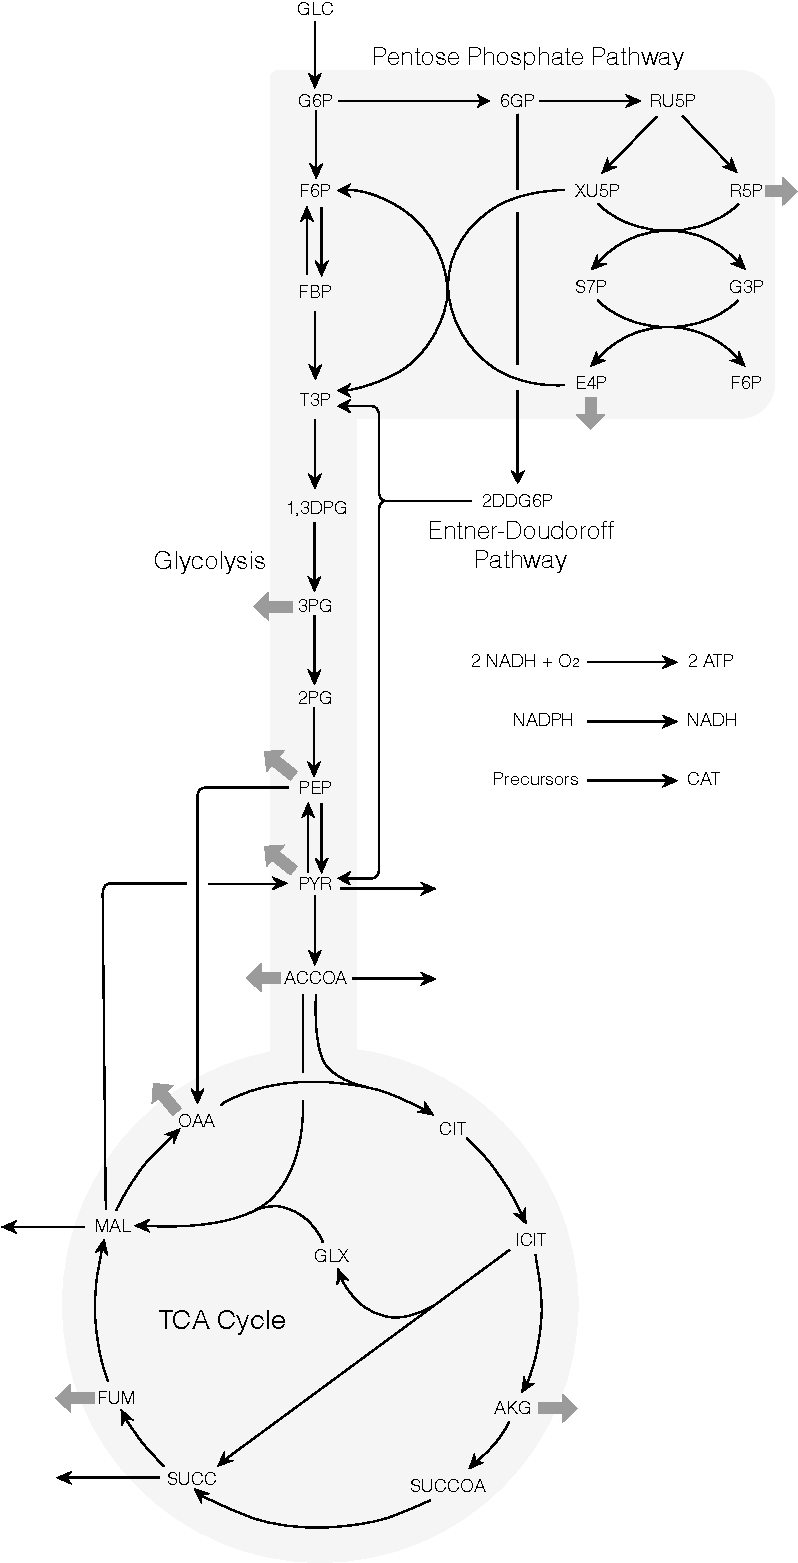
\includegraphics[width=0.75\textwidth]{./Figures/Network.pdf}
\caption{Flux profile for glycolysis, pentose phosphate pathway, Entner-Doudoroff pathway, TCA cycle, and NADPH/NADH transfer. FBA flux value (top), and mean ± standard error across ensemble at 1.5 hrs (middle) and 3 hrs (bottom), normalized to CAT synthesis flux.}
\label{fig:Network}
\end{figure}

\begin{figure}[ht]
\centering
%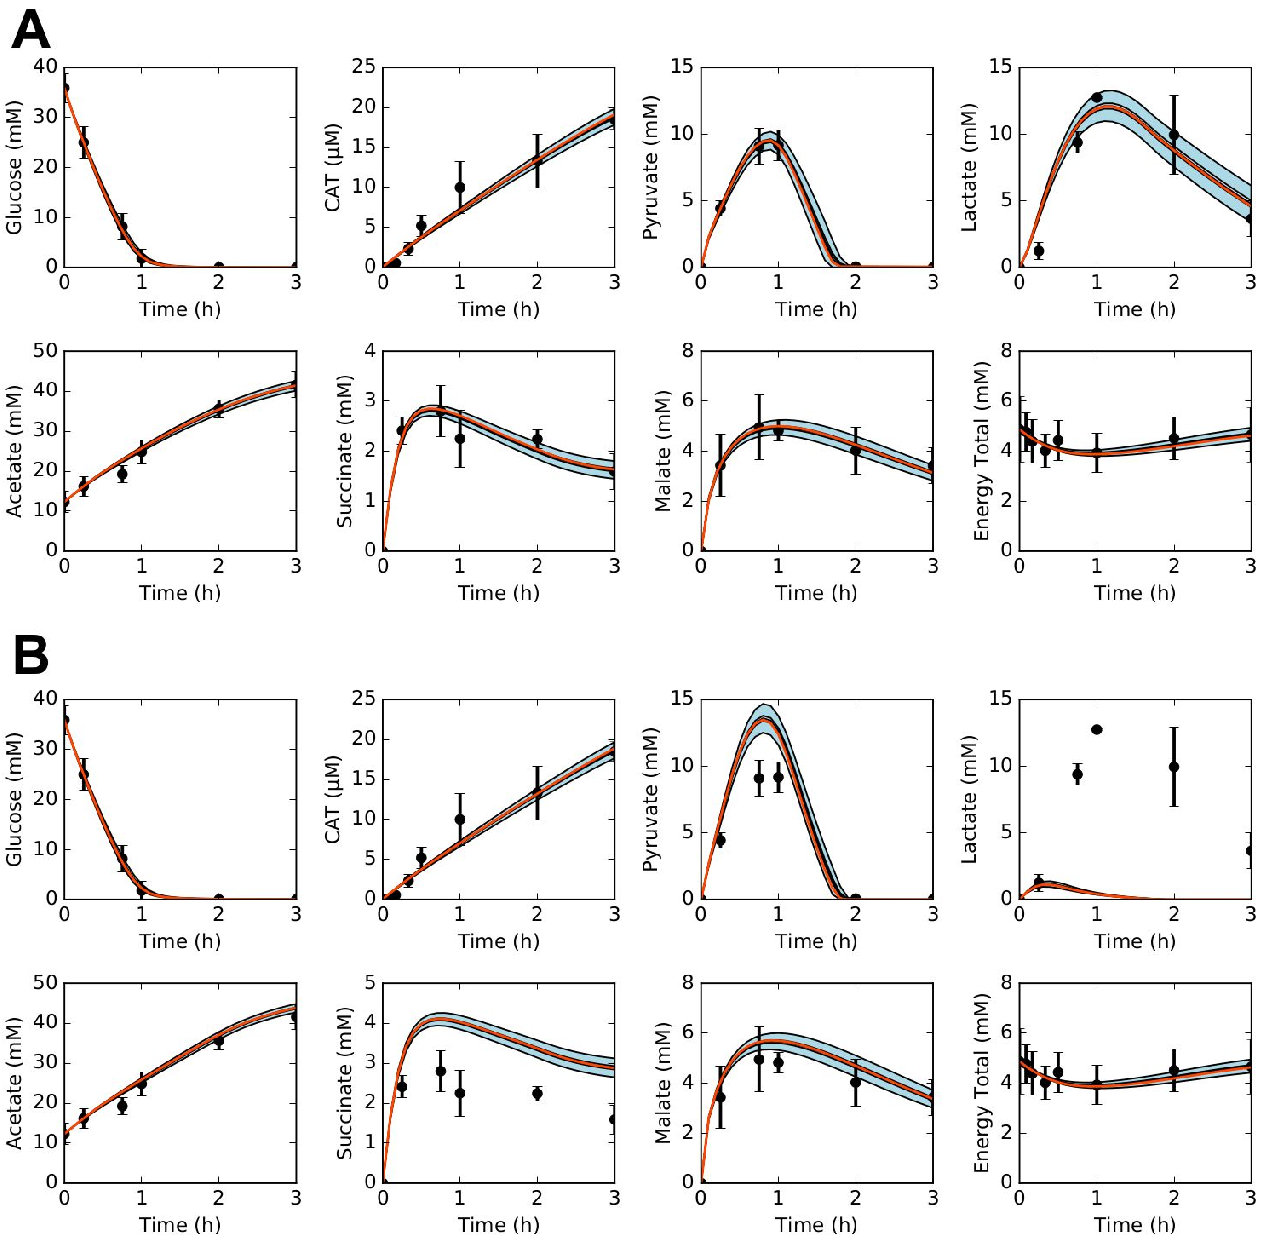
\includegraphics[width=1.00\textwidth]{./Figures/BothCarbon.pdf}
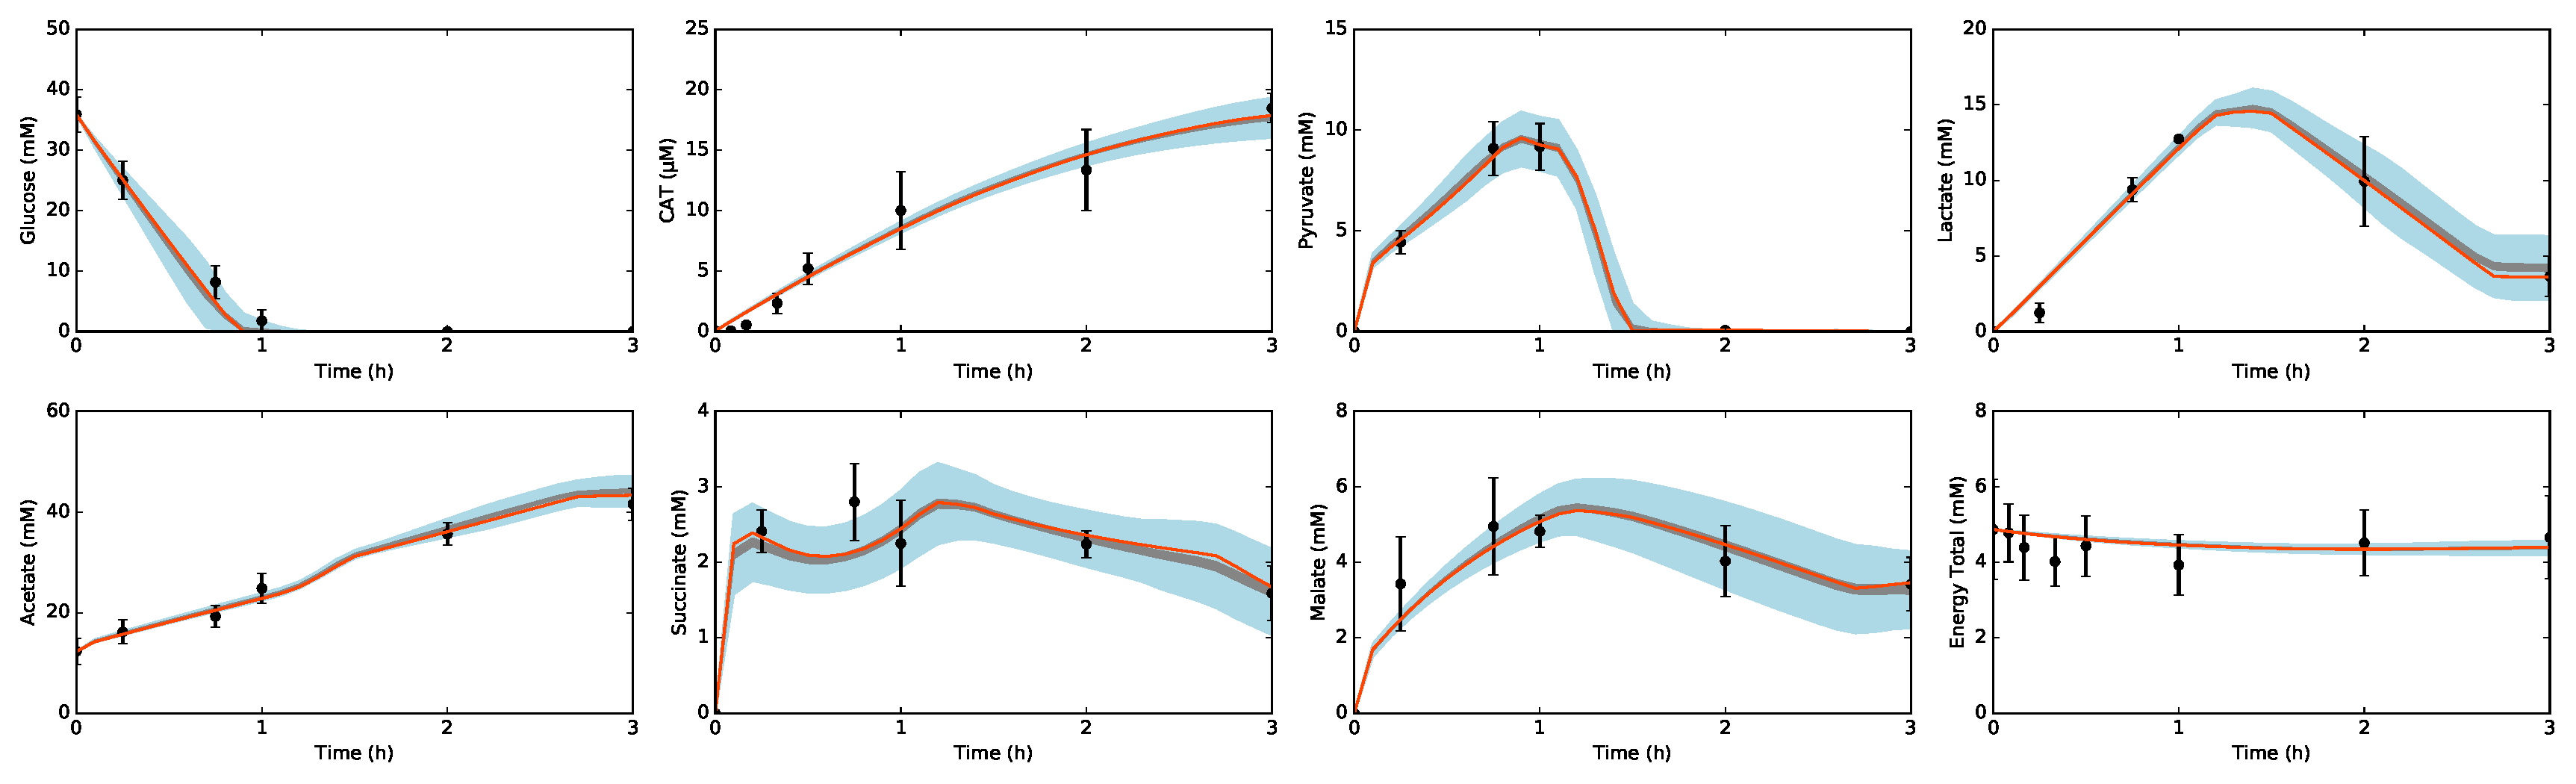
\includegraphics[width=1.00\textwidth]{./Figures/Carbon.pdf}

\includegraphics[width=0.05\textwidth]{./Figures/null.pdf}
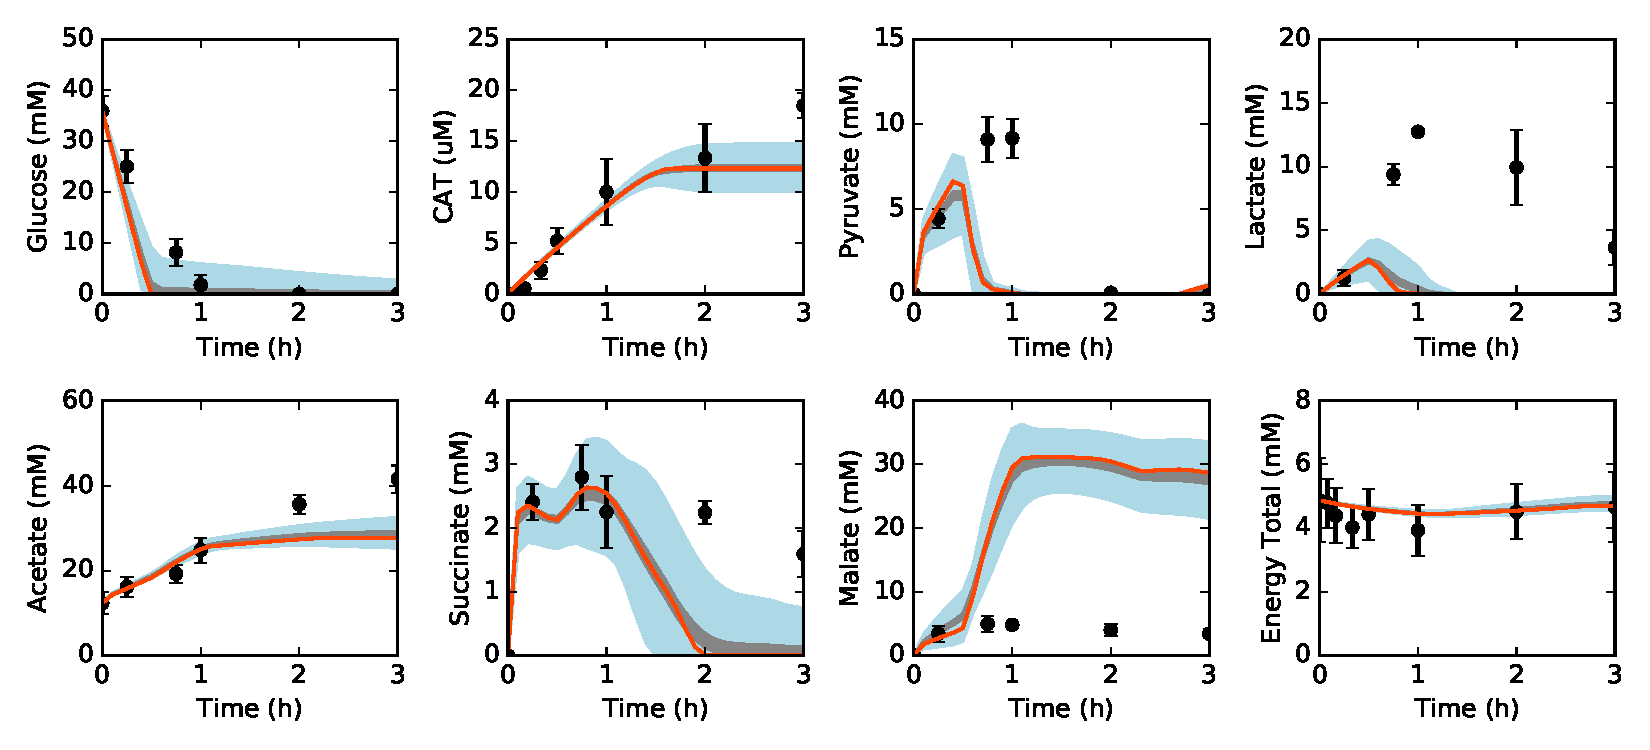
\includegraphics[width=1.00\textwidth]{./Figures/CarbonNoControl.pdf}
\caption{Central carbon metabolism in the presence (top) and absence (bottom) of allosteric control, including glucose (substrate), CAT (product), and intermediates, as well as total concentration of energy species. Best-fit parameter set (orange line) versus experimental data (points). 95\% confidence interval (blue shaded region) and 95\% confidence interval of the mean (gray shaded region) over the ensemble of 18,000 sets.}
\label{fig:BothCarbon}
\end{figure}

\begin{figure}[ht]
\centering
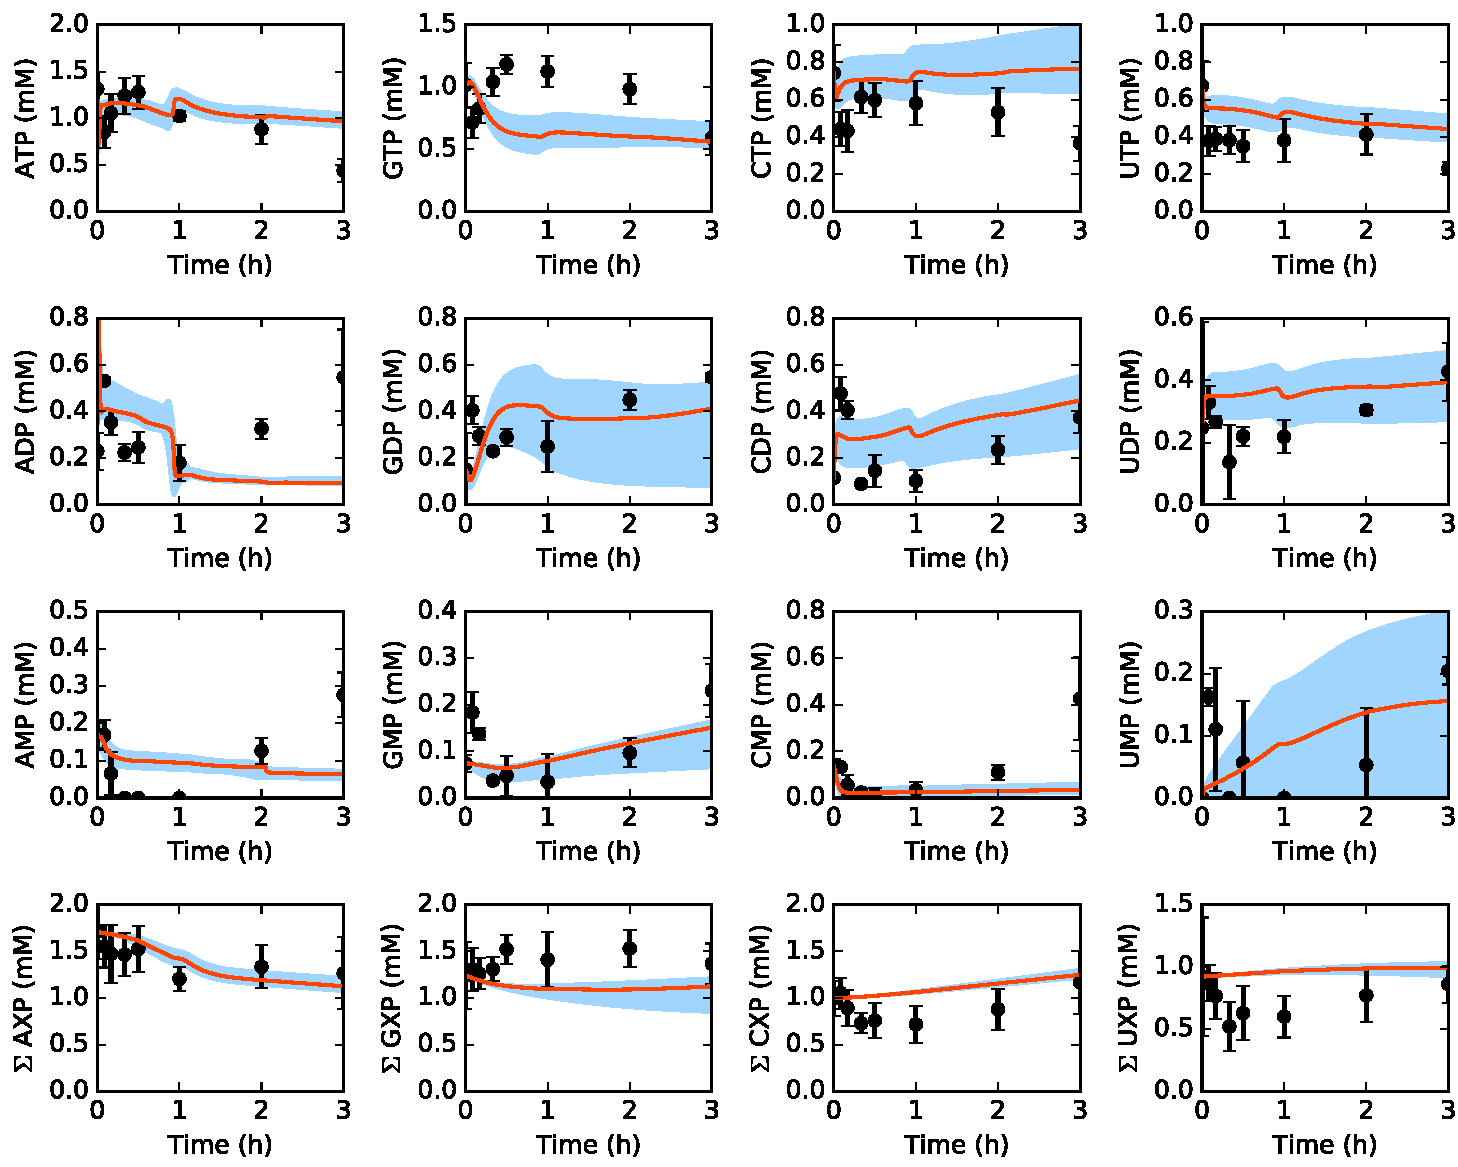
\includegraphics[width=1.00\textwidth]{./Figures/Energy.pdf}
\caption{Energy species and energy totals by base in the presence of allosteric control. Best-fit parameter set (orange line) versus experimental data (points). 95\% confidence interval (blue shaded region) and 95\% confidence interval of the mean (gray shaded region) over the ensemble of 18,000 sets.}
\label{fig:Energy}
\end{figure}

\begin{figure}[ht]
\centering
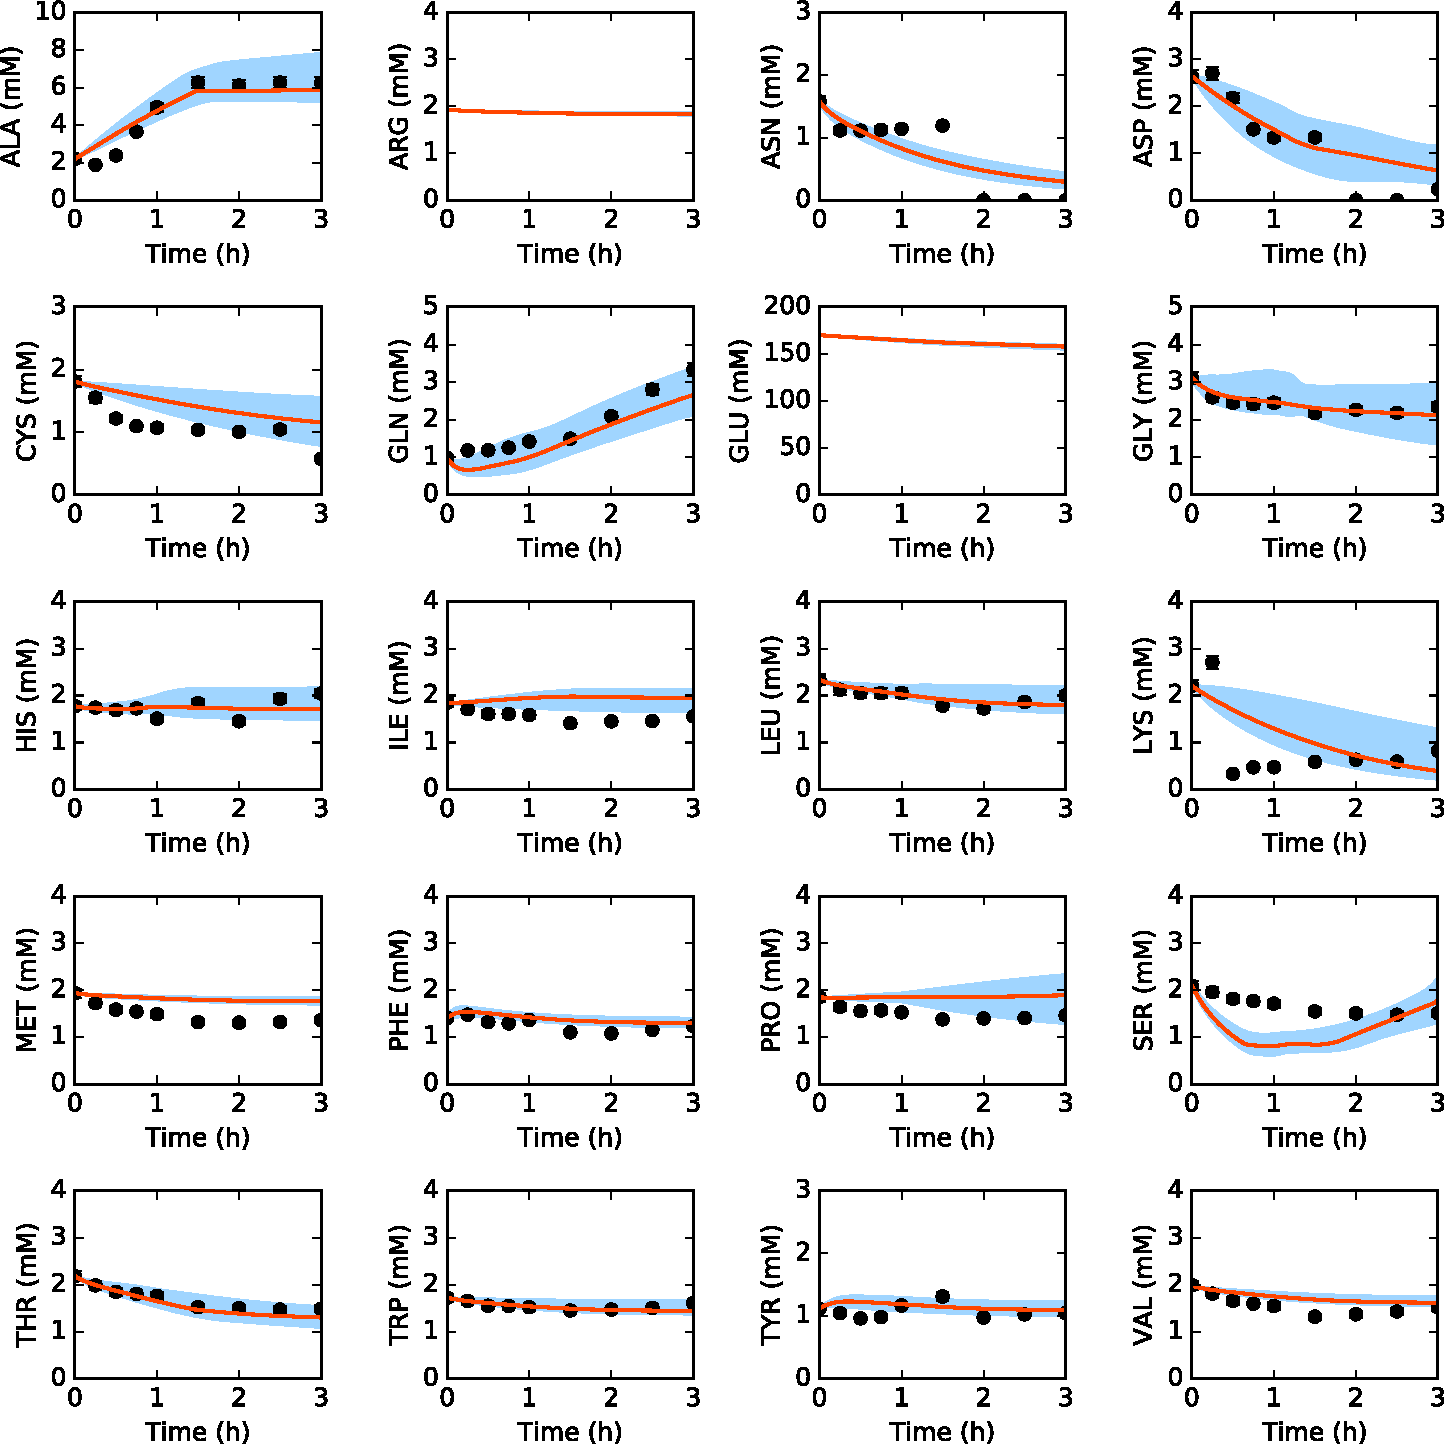
\includegraphics[width=1.00\textwidth]{./Figures/Amino.pdf}
\caption{Amino acids in the presence of allosteric control. Best-fit parameter set (orange line) versus experimental data (points). 95\% confidence interval (blue shaded region) and 95\% confidence interval of the mean (gray shaded region) over the ensemble of 18,000 sets.}
\label{fig:Amino}
\end{figure}

\begin{figure}[ht]
\centering
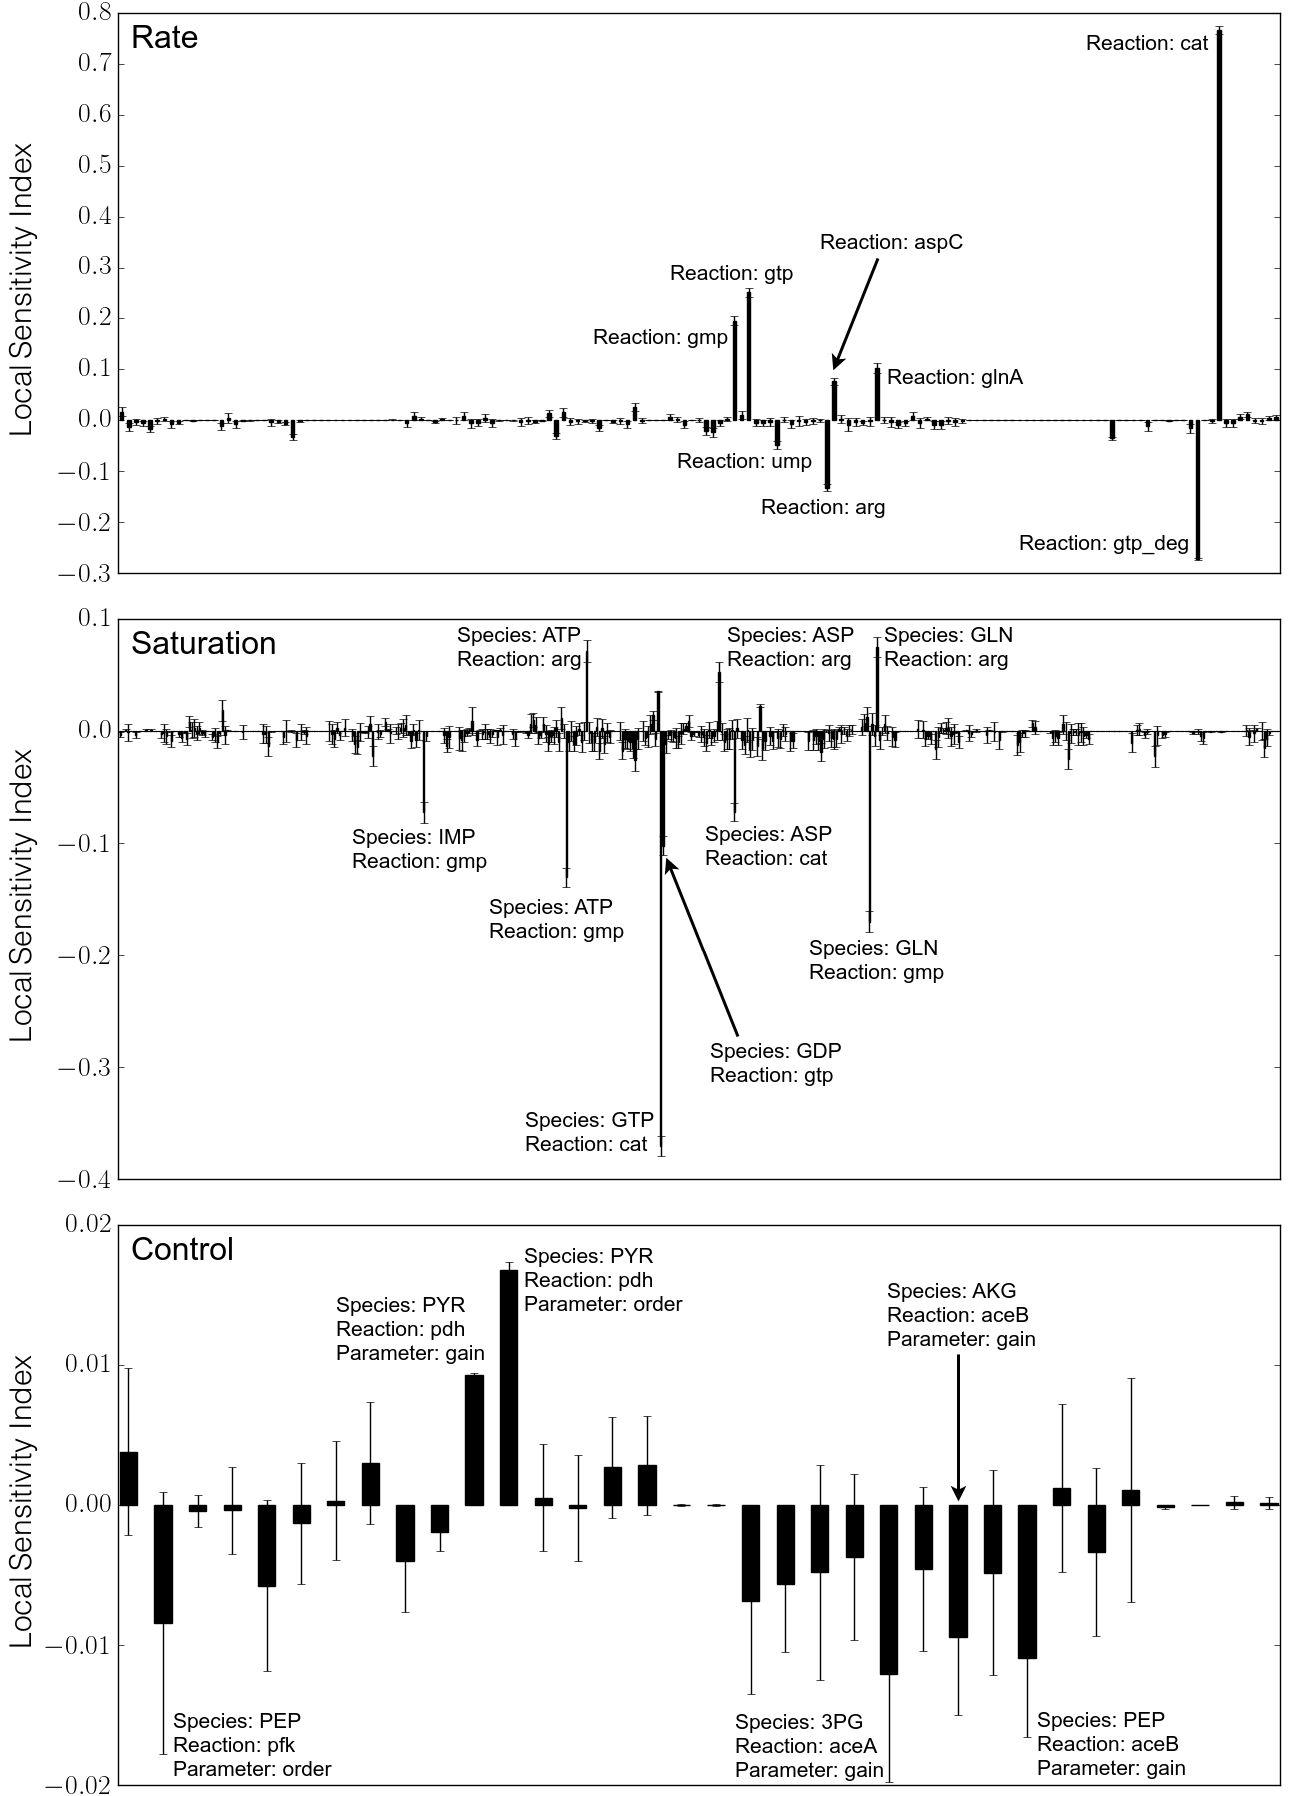
\includegraphics[width=0.94\textwidth]{./Figures/SensAll.png}
\caption{Mean and standard error of local sensitivities of rate constants (top), saturation constants (middle), and control parameters (bottom).}
\label{fig:LocalSensitivity}
\end{figure}

\begin{figure}[ht]
\centering
%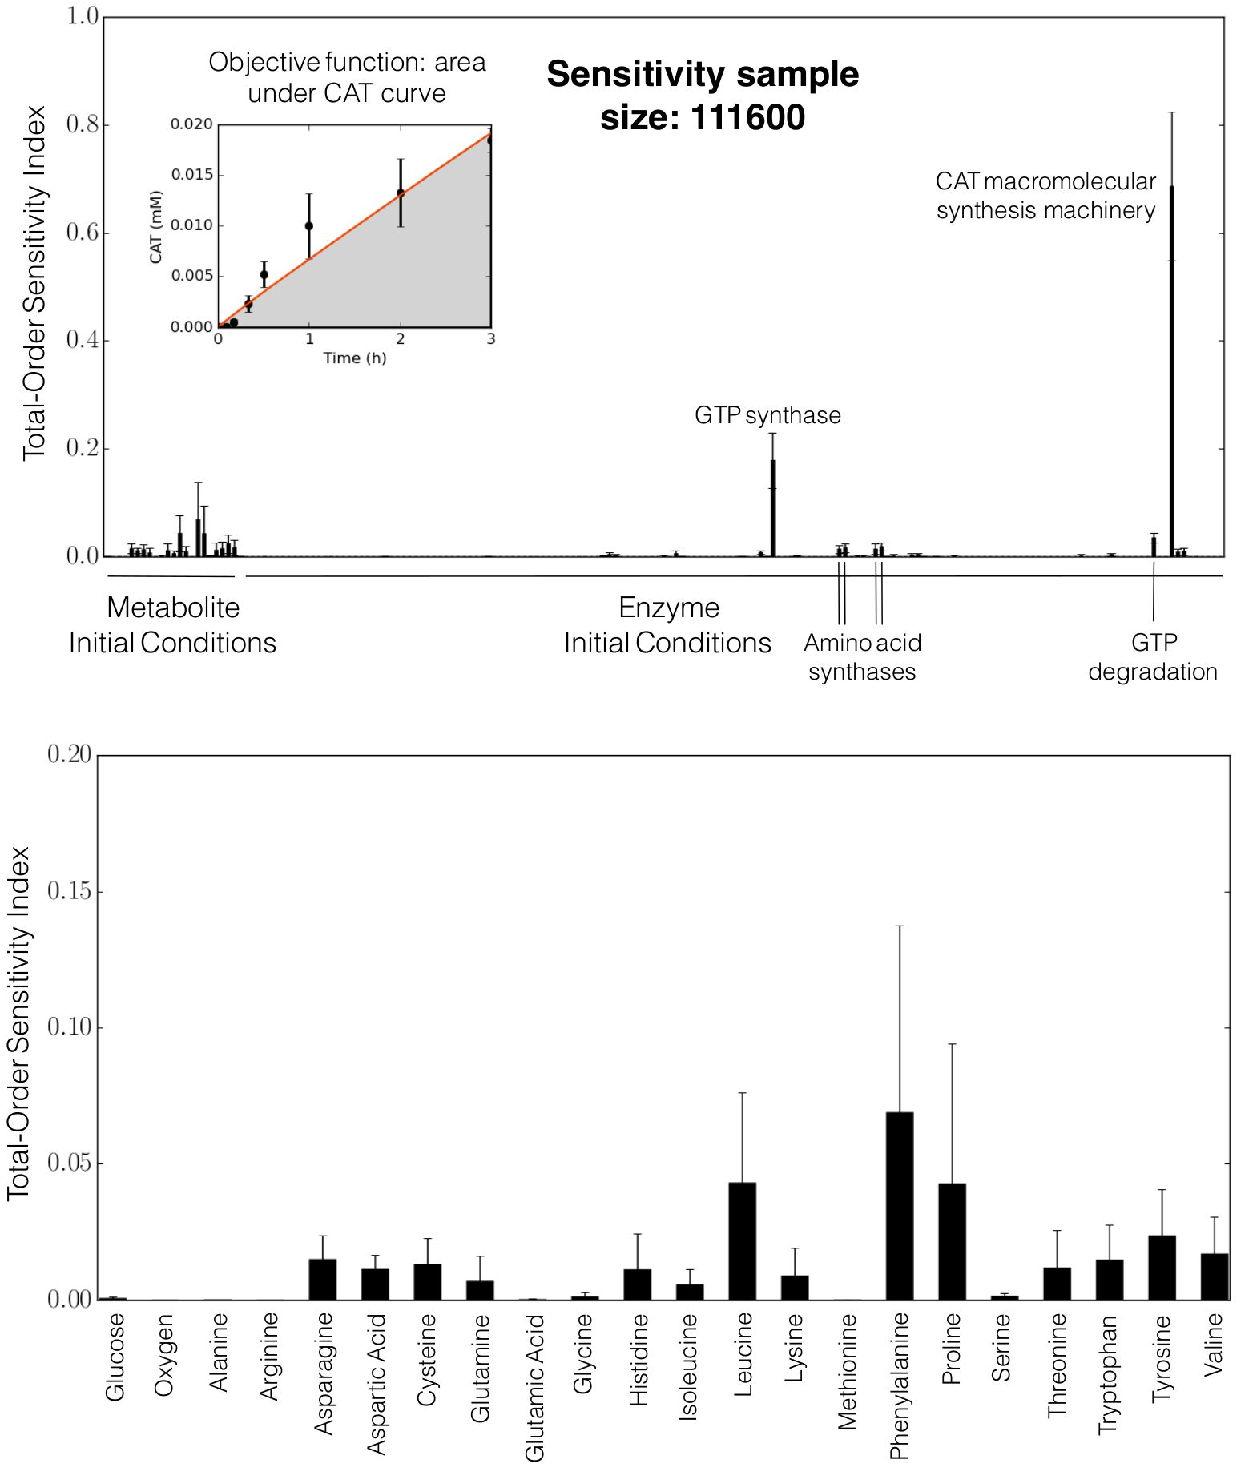
\includegraphics[width=1.00\textwidth]{./Figures/SensitivitiesHalfTall.pdf}
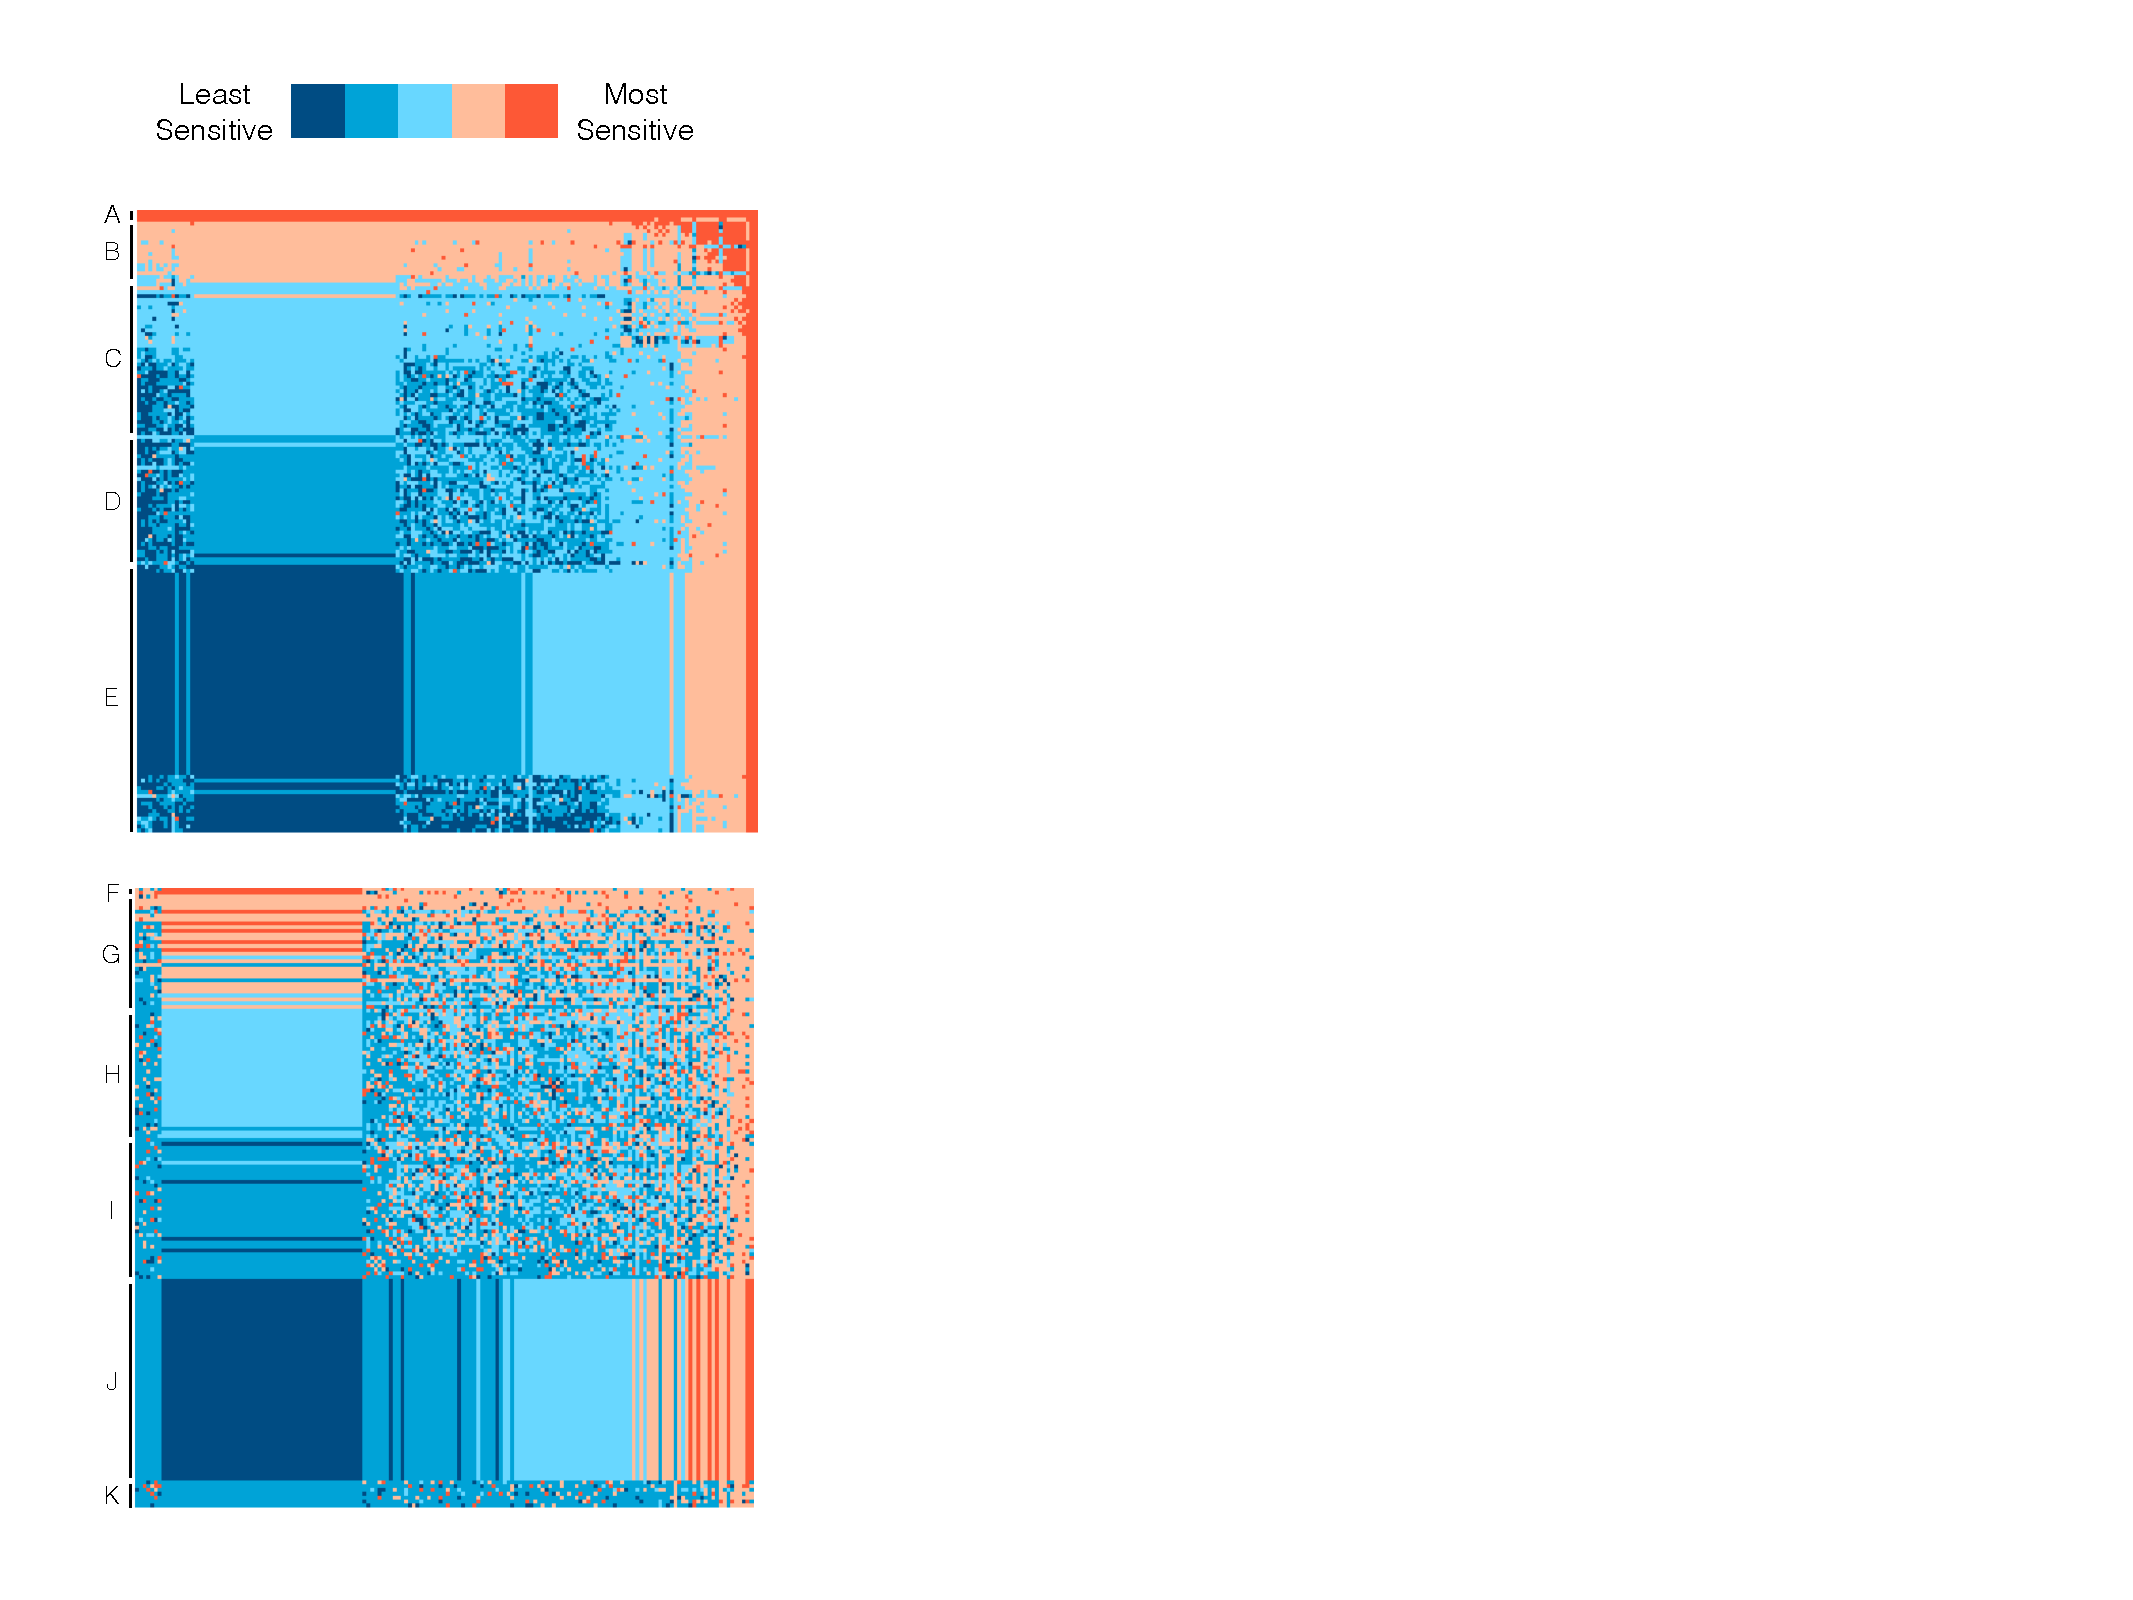
\includegraphics[width=1.00\textwidth]{./Figures/Sensitivity.pdf}
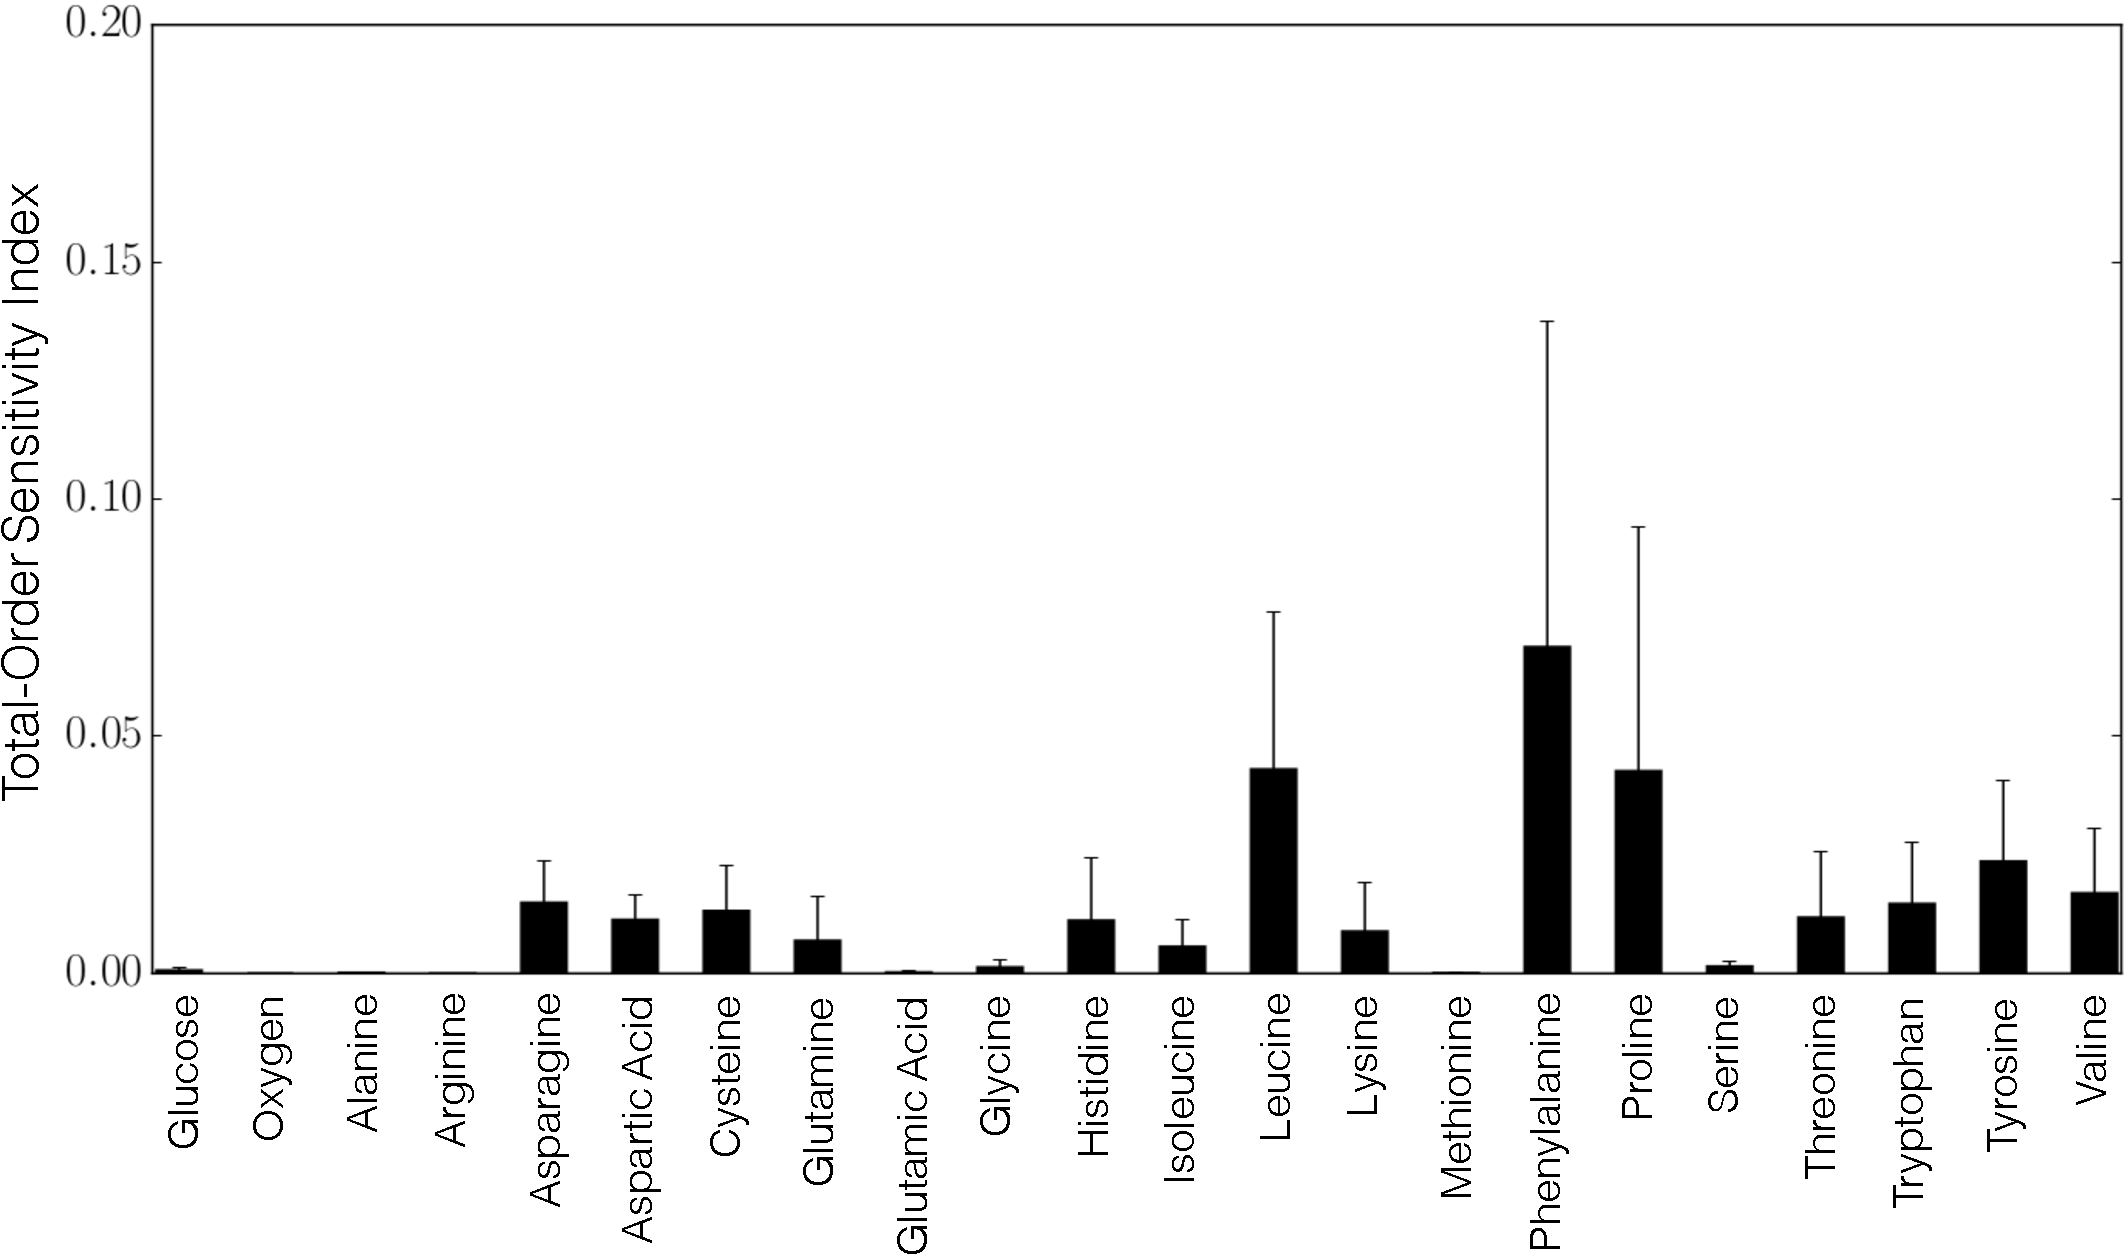
\includegraphics[width=1.00\textwidth]{./Figures/Metab_sensitivity.pdf}
\caption{Total-order global sensitivities for experimentally controllable initial conditions, including glucose, oxygen, amino acids, and enzymes.}
\label{fig:GlobalSensitivity}
\end{figure}

\clearpage

% Supplemental figures -
% Set the S-
\renewcommand\thefigure{S\arabic{figure}}
\renewcommand\thetable{T\arabic{table}}
\renewcommand\thepage{S-\arabic{page}}
\renewcommand\theequation{S\arabic{equation}}

% Reset the counters -
\setcounter{equation}{0}
\setcounter{table}{0}
\setcounter{figure}{0}
\setcounter{page}{1}


% Supplemental figures go here ...
%\begin{figure}[ht]
%\centering
%\includegraphics[width=1.00\textwidth]{./figs/<Filename>.pdf}
%\caption{Captiontext goes here}
%}\label{fig:<label_name>}
%\end{figure}

\end{document}
